\chapter{Fejlesztői dokumentáció I: A NES működésének ismertetése} % Developer guide
\label{ch:impl}

\section{A NES felépítése}

\begin{figure}[H]
	\centering
	\includegraphics[scale=0.19]{mobo.jpg}
	\caption{A NES alaplapja\protect\footnotemark}
\end{figure}

\footnotetext{\url{https://commons.wikimedia.org/wiki/File:Nintendo-NES-Mk1-Motherboard-Top.jpg}}
Ennek az ismertetőnek az a célja, hogy az olvasó magas szinten átlássa a NES legfontosabb egységeinek működését. A mélyebb megértéshez a forráskód tanulmányozását, valamint a \emph{Nesdev}\cite{ref} oldalt ajánlom.
A NES emulációjához az alábbi komponenseket kellett megismernem, amik közül a CPU és a PPU működését fogom később részletesebben áttekinteni.

\begin{compactdesc}
	\item[Ricoh RP2A03:] 
	\hfill \\
	A hangchipet és központi feldolgozóegységet (CPU) tartalmazó integrált áramkör. Utóbbi nem más, mint az Apple II-ben és Commodore 64-ben használt 8-bites MOS Technology 6502.
	\item[Ricoh RP2C02:]
	\hfill \\
	A képfeldolgozó egység, rövid nevén PPU (Picture Processing Unit).
	\item[NROM\cite{nromref}, UNROM\cite{unromref} és CNROM\cite{cnromref}:] 
	\hfill \\
	Az emulátor által támogatott három kazettatípus.
	\item[Sztenderd NES kontroller\cite{control}:]
	\hfill \\
	A konzol alapértelmezett beviteli eszköze.
\end{compactdesc}

\section{Órajel-frekvenciák \cite{nesclocks}}
A párhuzamosan működő komponenseket az órajelek hangolják össze. Az órajel-frekvencia határozza meg, hogy egy másodperc alatt hány atomi műveletet végez el egy komponens.
A CPU és a PPU is rendelkezik saját órajelfrekvenciával, amit egy központi órajelből származtatnak.

\begin{itemize}
	\item Központi órajel-frekvencia: $ f = \frac{236.25\;MHz}{11} \sim 21.477272\; MHz $
	\item CPU órajel-frekvencia: $ \frac{f}{12} \sim 1.789773 \; MHz  $
	\item PPU órajel-frekvencia: $ \frac{f}{4}  \sim 5.369318 \; MHz $
\end{itemize}

\section{A központi feldolgozóegységhez kapcsolódó fogalmak}

\begin{note}
	A hexadecimális értékeket \textbf{\$} prefix-el jelölöm.
\end{note}

\subsection{Opkód \cite{6502desc} \cite{6502opc}}
Egy opkód a 6502 esetében csupán egyetlen bájt, amiből az utasításdekódoló egyértelműen meg tudja határozni a végrehajtandó utasítást és annak címzési módját.
Ezt a hozzárendelést az opkódmátrix írja le. Az emulációhoz emellett azt is tárolni kell az opkódmátrixban, hogy a végrehajtandó művelet hány CPU-órajel alatt fejeződik be, ugyanis csak ennek ismeretében tudjuk a CPU-t és a PPU-t precízen egymáshoz szinkronizálni.

\begin{figure}[H]
	\centering
	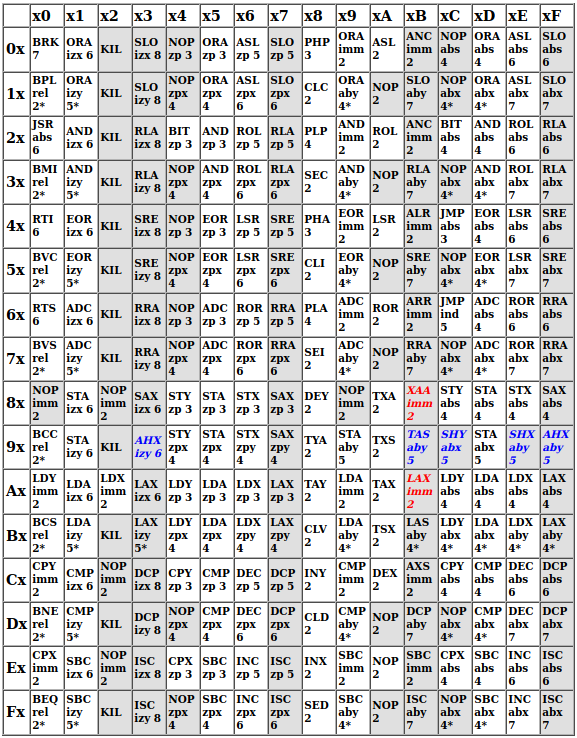
\includegraphics[scale=0.65]{opcodes.png}
	\caption{A 6502 opkódmátrixa}
	\label{fig:opcodes}
\end{figure}

Ha meg szeretnénk találni egy adott opkódhoz a hozzá tartozó információt, akkor szükségünk lesz az opkód hexadecimális alakjára, ami legfeljebb kétszámjegyű lehet. A nagyobb helyiértékű számjegy a keresett cella sorát, a kisebbik pedig az oszlopát írja le. Példaként a \ref{fig:opcodes} ábrán láthatjuk, hogy a \$30 opkódhoz a BMI utasítás tartozik relatív címzéssel.
Azok az opkódok csillaggal vannak jelölve, amiknek a futási ideje megnőhet az aktuális argumentumoktól függően.
A szürkével jelölt opkódokhoz hivatalosan nincs utasítás rendelve. 
Ezeket a nem dokumentált, ``illegális'' opkódokat a processzor későbbi 
verzióinak hagyták fent. \cite{illegal} A tervezők nem tiltották meg azonban ezeknek a használatát, 
egyszerűen csak nem definiálták a viselkedésüket. Ennek ellenére több olyan illegális opkód is belekerült a dizájnba, ami később hasznosnak bizonyult. A játékfejlesztők próbálkozások útján
felfedezték, hogy melyek azok az opkódok, amiknek a viselkedése determinisztikus és néhány speciális feladat esetén érdemes őket használni.
Ritka ugyan, de van olyan játék, ami ezeket az opkódokat is használja, ezért ezeknek az opkódoknak az emulációját is megvalósítottam.

\subsection{Regiszterek \cite{6502desc}}
A regiszter a processzor leggyorsabban elérhető memóriája.
A gyártási költségek alacsonyan tartása végett csak 6 regiszter került a processzorba.
Minden regiszter mellett zárójelben fel van tüntetve annak mérete bitekben megadva.

\begin{compactdesc}
	\item[A (8):] Akkumulátor, az aritmetikai műveletek eredményei ebbe kerülnek.
	\item[X (8) és Y (8):] 
	Index regiszterek, indirekt címzésnél használjuk őket.
	Ciklusok esetén a ciklusváltozót érdemes ezekben tárolnunk.
	\item[S (8):] 
	Verem mutató. A verem tetejének a kezdőcímtől vett eltolását tárolja.
	\item[P (8):]
	Státusz regiszter, ami 7 darab flag bitet tárol.
	\item[PC (16):]
	Programszámláló. 
	A következő opkód memóriacímét tárolja.
	Méretéből következik, hogy a processzor teljes címtartománya 64 KiB nagyságú.
\end{compactdesc}


\subsection{Memórialap}
Az $i$. lap egy 256 bájtos egybefüggő memóriarész, ami a $ [i \cdot \$100, \: (i+1) \cdot \$100) $ címtartományon helyezkedik el.

\subsection{Hívási verem \cite{6502desc} \cite{6502instr}}
Az egymásba ágyazott eljárásokat a processzor hardveresen támogatja, amihez a vermet használja.
A verem az 1. lapon található, és a kisebb címek felé nő.
Eljárás hívásakor a verem tetejére kerül az aktuális programszámláló értéke, 
visszatéréskor pedig a veremről levett címre állítjuk be a programszámláló értékét.

\subsection{Megszakítás \cite{6502desc} \cite{cpumem}}
A komponensek kommunikációjának egyik módja a hardveres megszakítás.
A 6502 chip egy darab maszkolható \emph{(IRQ)} és egy nem maszkolható \emph{(NMI)} megszakítási lábbal rendelkezik.
A megszakítási vektorokkal a program beállíthatja, hogy egy bizonyos megszakításra milyen szubrutinnal kíván reagálni. A vektorok 2 bájtos tárolók, amik a kezelő szubrutin címét tartalmazzák. Az NMI-hez tartozó vektor a \$FFFA és a \$FFFB címeken, míg az IRQ-hoz tarozó vektor az \$FFFE és a \$FFFF címeken található. A 6502 ``kicsi az elején'' bájtsorrendű (little-endian) processzor, ezért a címeknek mindig az alsó 8 bitjét tárolja az alacsonyabb címen, a felső 8 bitjét pedig a magasabb címen.
A program dönthet úgy, hogy a maszkolható megszakítást figyelmen kívül hagyja (a kezelő szubrutin nem hívódik meg), ehhez az \emph{IRQ Disable} flag-et be kell állítania a státusz regiszterben. A nem maszkolható megszakítás esetén erre nincsen lehetőség, a végrehajtás mindenképpen a kezelő szubrutinhoz ugrik.
A nem maszkolható lábhoz a képfeldolgozó, a maszkolhatóhoz a hangchip van kötve.

\subsection{Opkód argumentum helye, fajtája}

\begin{figure}[H]
	\centering
	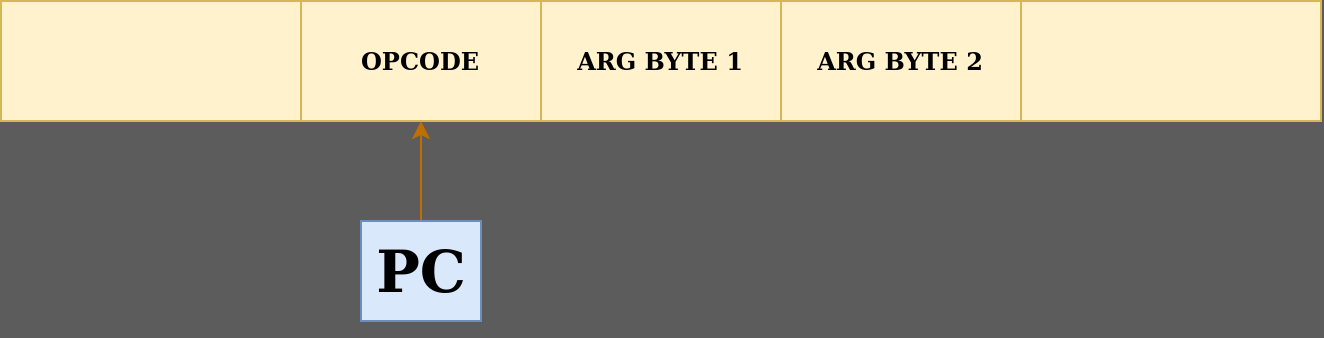
\includegraphics[scale=0.25]{opcode.png}
	\caption{Opkód argumentumainak helye}
	\label{fig:argplacement}
\end{figure}

A \ref{fig:argplacement} ábra szemlélteti, hogy az opkód argumentumok közvetlenül az opkód mögött, a \emph{PC+1} és \emph{PC+2} címeken helyezkedhetnek el a memóriában. Címzési módtól függően változhat az argumentumok száma 0, 1 és 2 bájt között.
Ha az opkód rendelkezik argumentummal vagy argumentumokkal, akkor azok a következő fajtájúak lehetnek:

\begin{compactitem}
	\item 2 bájt, ami abszolút memóriacímet ábrázol kicsi-az-elején bájtsorrenddel 
	\item 1 bájt, ami relatív eltolást ír le
	\item 1 bájt, ami a művelet közvetlen operandusa
\end{compactitem}

\subsection{Címzési módok \cite{6502desc} \cite{cpuref}}

Egy opkód után azoknál a címzési módoknál áll argumentum, amiknél a művelet elvégzéséhez 
szükséges operandus nem regiszterben, hanem a memóriában van. A címzési módok azt határozzák meg, hogy az argumentumból hogyan kell kiszámolni az operandus effektív 16 bites memóriacímét. Az alábbiakban felsorolt  címzési módoknál a zárójelben az opkódmátrixbeli név (amennyiben van) és az argumentum bájtok száma található.  


\begin{description}
	\item[Akkumulátor mód (0):] nincs argumentum, az utasítás az \textbf{A} regiszter értékét módosítja.
	\item[Azonnali mód (imm, 1):] az utasítás operandusa maga az argumentum. Jele: \#
	\newline
	Példa: az LDA \#\$0 utasítás nullára állítja az \textbf{A} regisztert.
	\item[Abszolút mód (abs, 2):] az argumentum az operandus effektív címe.
	\item[0. lap mód (zp, 1):] A CPU kevés regiszterét azzal ellensúlyozták, hogy ennek a speciális módnak köszönhetően a nulladik lapot hatékonyabban lehet címezni, mint a többit. 
	Mivel a 0. lap mérete 256 bájt, ezért teljes cím helyett elég egyetlen bájt a címzéséhez.
	A kisebb paraméter gyorsabban beolvasható és egyúttal a kódméretet is csökkenti.
	\item[Indexelt 0. lap mód (zpx, zpy, 1):]
	Hasonlóan most is csak a 0. lapot tudjuk címezni, de az argumentumhoz hozzáadjuk valamelyik index regiszter értékét.
	Az operandus címének kiszámítása: $ (arg1 + index) \mod 256 $
	\item[Indexelt abszolút mód (abx, aby, 2):] Az argumentumok egy teljes memóriacímet alkotnak, amihez hozzáadjuk a megadott index regiszter értékét. 
	\item[Implicit mód (0):] nincs szükség argumentumra, mert az utasítás regiszterekkel dolgozik.
	\item[Relatív mód (rel, 1):] Az elágazási utasítások használják ezt a címzési módot. Elágazásoknál, ha a feltétel teljesül, akkor az argumentummal el kell tolni a programszámlálót. Az elágazási utasítások feltételeit lásd az \emph{\nameref{instructionset}} szekcióban.
	\item[Indirekt mód (ind, 2):] 
	Erre a címzési módra a JMP utasításnál van szükség.
	A két argumentum bájt együtt egy teljes memóriacímet alkot, legyen ez \emph{m}.
	Az operandus címét az \emph{m} és \emph{m+1} címeken találjuk, így tehát az operandus értékét a következő módon kapjuk meg: $$ operand := read(\;(read(m+1) << 8) \;\; | \;\; read(m)\;) $$
	\item[Indexelt indirekt mód (izx, 1):]
	Az X regisztert összeadjuk az argumentummal, így egy 0. lapon található címet kapunk.
	Erről a címről kell az operandus effektív címét kiolvasni.
	\begin{figure}[H]
		\centering
		\vspace{0.4cm}
		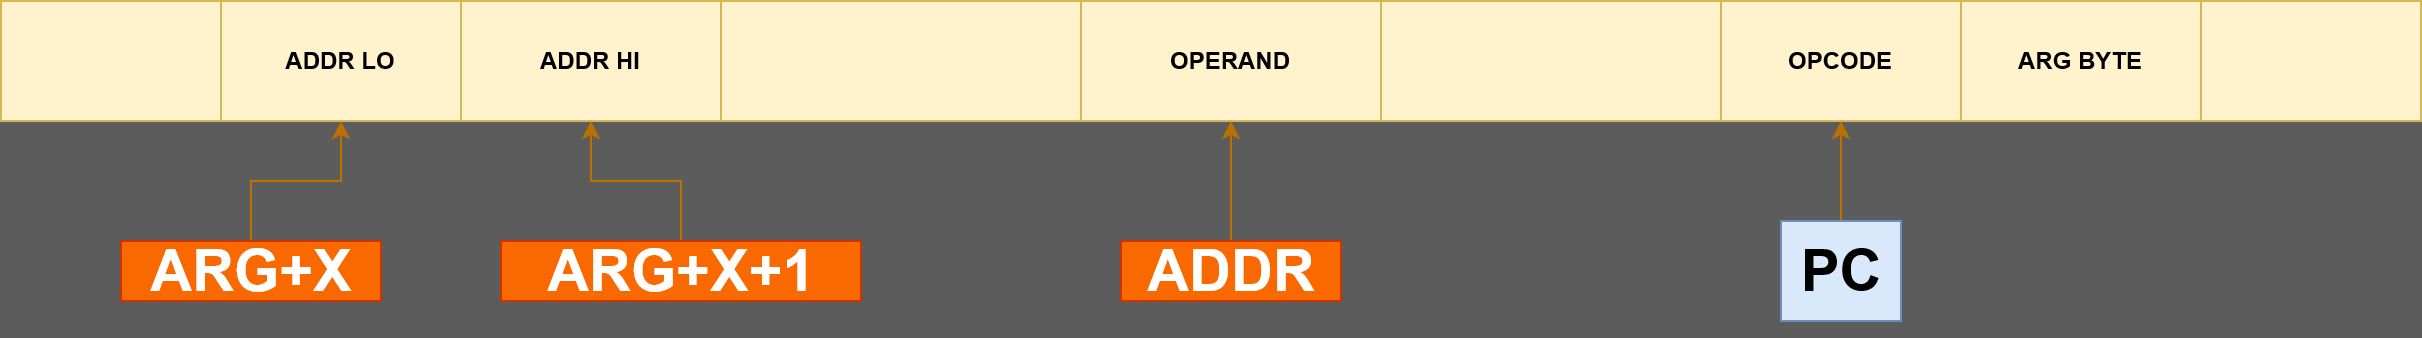
\includegraphics[width=1.1\textwidth,height=70px]{indexed_indirect.png}
		\caption{Indexelt indirekt címzés}
	\end{figure}
	\item[Indirekt indexelt mód (izy, 1):]
	Az argumentum egy 0. lapon található címre mutat, amit ha összeadunk az Y regiszter értékével, akkor megkapjuk az operandus effektív címét. 
	
	
	
\end{description}

Az \textbf{abx}, \textbf{aby} és \textbf{izy} indexelt címzési módok és bizonyos utasítások kombinációjánál előfordulhat, hogy a végleges operandus cím és az indexelés előtt álló cím különböző memórialapra esik. Ebben az esetben 1 órajelciklussal tovább tart az utasítás végrehajtása.
Emellett az elágazási utasítások (relatív címzés) több ciklus alatt fejeződnek be, ha az ugrási feltétel teljesül. Ha az ugrás előtti PC értéke és az ugrási cél más lapra esik, akkor +2, ellenkező esetben csak +1 órajelciklussal kell számolni.

\subsection{Memóriatérkép \cite{cpumem}}

A memóriatérkép leírja a címtér felosztását a komponensek között.
A memóriatérképből meg tudjuk állapítani, hogy egy adott címen található bájt kiolvasásához vagy írásához melyik komponens hardveres logikáját kell alkalmazni.

\begin{table}[H]
	\centering
	\begin{tabular}{ | l | l | }
		\hline
		Tartomány & Eszköz \\
		\hline			
		$ \$0000 - \$07FF $ & CPU RAM \\
		$ \$0800 - \$1FFF $ & CPU RAM tükrözése \\
		$ \$2000 - \$2007 $ & PPU regiszterek \\
		$ \$2008 - \$3FFF $ & PPU regiszterek tükrözése \\
		$ \$4000 - \$4017 $ & APU és IO regiszterek \\
		$ \$4018 - \$401F $ & APU és IO regiszterek tükrözése \\
		$ \$4020 - \$FFFF $ & Kazetta \\
		\hline
	\end{tabular}
\end{table}

\subsection{Memóriatükrözés \cite{memmirror}}
Memóriatükrözésről beszélünk, amikor fizikailag ugyanazt a memóriaterületet több memóriacímről is el tudjuk érni. Ha egy címtartomány $x$ bájtonként tükrözve van, akkor minden olyan $a$ és $b$ memóriacím ugyanarra a bájtra mutat, ami a tartományba vagy a tükrözésébe esik és $a \equiv b\ (\textrm{mod}\ x)$.  A CPU RAM 2 KiB-onként tükrözve van, amiből következik, hogy a \$0001, \$0801 \$1001, \$1801 címek ugyanarra a bájtra mutatnak. Egy címtartomány tükrözése lehet nagyobb mint az eredeti tartomány (például a CPU RAM esetében a tükrözési tartomány háromszor nagyobb).

\subsection{Státusz flagek}

\begin{compactenum}
	\setcounter{enumi}{-1}
	\item bit: C = Carry \newline Összeadások, forgatások, eltolások során a leeső biteket jelzésére.
	\item bit: Z = Zero   \newline Aritmetikai művelet eredménye vagy mozgatott bájt 0.
	\item bit: I = IRQ Disable
	\newline Az 1-re állításával maszkoljuk az IRQ-t.
	\item bit: D = Decimal mode
	\newline
	A NES nem használja ezt a flag-et.
	\item bit: B = BRK Command
	\newline Az 1-re állításával generálhatunk egy szoftveres megszakítást. 
	\setcounter{enumi}{5}
	\item bit: V = Overflow
	\newline 
	Aritmetikai műveleteknél a túlcsordulás vagy alulcsordulás jelzésére.
	A BIT utasítás speciálisan használja.
	\item bit: N = Negative
	\newline A manipulált bájt negatív, vagyis a legnagyobb helyiértékű bitje 1.
\end{compactenum}

\subsection{Utasításkészlet \cite{6502desc} \cite{6502opc} \cite{6502instr}}
\label{instructionset}

\begin{compactdesc}
	\item Aritmetikai és logikai egység (ALU) \hfill \\
	\textbf{ADC:} Összeadás;
	\textbf{SBC:} Kivonás;
	\textbf{AND:} Logikai ÉS művelet;
	\textbf{ASL:} Bájt balra elcsúsztatása;
	\textbf{LSR:} Bájt jobbra elcsúsztatása;
	\textbf{ORA:} Logikai VAGY;
	\textbf{EOR:} Kizárásos VAGY;
	\textbf{INC, INX, INY:} növelés eggyel;
	\textbf{DEC, DEX, DEY:} csökkentés eggyel;
	\textbf{ROL, ROR:} bájt forgatása;
	\item 
	Összehasonlítás, tesztelés
	\begin{compactdesc}
		\item[CMP, CPX, CPY:]  \hfill \\ A megadott címen található bájt és rendre az A, X és Y regiszterekben található bájt között az $=$ és a $>=$ reláció kiértékelése
		\item[BIT:] Az operandus bájt maszkolása (\&) az A regiszter tartalmával, az eredmény szerint a Z,N,V flag-ek frissítése 
	\end{compactdesc}
	\item Veremműveletek
	\begin{compactdesc}
		\item[PHA:] Az akkumulátor regiszter értékének felrakása a veremre 
		\item[PHP:] A státusz regiszter értékének felrakása a veremre
		\item[PHA:] Az akkumulátor regiszter új értékének levétele a veremről
		\item[PHP:] A státusz regiszter új értékének levétele a veremről
	\end{compactdesc}
	\item Vezérlés
	\begin{compactdesc}
		\item[JMP:] Vezérlés áthelyezése egy megadott memóriacímhez, avagy a programszámláló átállítása erre a címre
		\item[JSR:] Szubrutin hívás (visszatérési cím elmentése + \textbf{JMP})
		\item[RTS:] Visszatérés szubrutinból (visszatérési cím kiolvasása + \textbf{JMP})
		\item[BRK:] Szoftveresen generált megszakítás
		\item[RTI:] Visszatérés megszakításkezelőből
	\end{compactdesc}
	\item Flag manipuláció (a utasításnév harmadik betűje a változtatott flag-et jelöli) \newline \textbf{CLC, CLD, CLI, CLV, SED, SEC, SEI}
	\newline
	(C = Clear, S = Set)
	\item Elágazások: vezérlés áthelyezése akkor, ha teljesül a feltétel az utasítás által vizsgált státusz flag-re
	\newline \textbf{BCC(C=0), BCS(C=1), BNE(Z=0), BEQ(Z=1), BPL(N=0), BMI(N=1),  BVC(V=0), BVS(V=1)}
	\item Bájtok mozgatása regiszterek és a memória között
	\newline
	\textbf{LDA, LDX, LDY, STA, STX, STY} 
	\newline
	(L = Load, S = Store)
	\newline
	A név harmadik betűje a használt regisztert jelöli.
	\item Bájtok mozgatása regiszterek között
	\newline
	\textbf{TAX, TAY, TSX, TXA, TXS, TYA}
	\newline
	A név második betűje a forrásregisztert, a harmadik a célregisztert jelöli.
\end{compactdesc}

\section{Kazetták \cite{ref}}

A kazettákon logikai szempontból kétfajta memória található: PRG és CHR.
PRG-ből lehet ROM és RAM is a kazettán. Ezekben a processzor által végrehajtandó utasítások, avagy a játéklogika kapott helyet. A CHR fajtáját tekintve ROM vagy RAM memória, amely a játék sprite-jait tárolja, amik 8*8 pixeles kis képekből állnak. Ezeket a kis képeket ezentúl alakzatoknak fogom hívni. 

\subsection{Az iNES fájlformátum \cite{ref} \cite{ines}}

Az iNES fájlformátumot egy korai NES emulátor vezette be a NES játékok bináris formában történő terjesztésére. A fájl elején található 16 bájtos fejléc többek között a mapper konfiguráció azonosítóját, a képfeldolgozó névtábláinak tükrözési módját, valamint a PRG ROM, PRG RAM és a CHR méretét határozza meg. A fejléc után ezek tartalma található.

\section{A képfeldolgozó egység}

\subsection{Színpaletta \cite{ppuref}}

A színpaletta hozzárendel egy $\$0$ és $\$3F$ közötti azonosítóhoz egy színkódot. A NES csak a színpaletta színeit tudja megjeleníteni (tehát 55 szín áll rendelkezésre). Egy pixel színét az fogja eldönteni, hogy milyen azonosító tartozik hozzá. A színpaletta fix, futás közben nem változtathatjuk meg a hozzárendelést.
\iffalse
\vspace{0.3cm}
\begin{figure}[H]
	\centering
	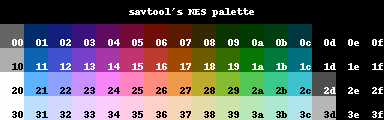
\includegraphics{palette.png}
	\caption{A 2C02 színpalettája}
\end{figure}
\clearpage
\fi

\subsection{Paletta indexek \cite{ppuref}}

A $\$3F00 - \$3F1F$ címtartományon található paletta index egy memóriacím $\rightarrow$ azonosító hozzárendelést ír le, azonban ezt a program már változtathatja futás során, mert RAM típusú memóriáról van szó. A paletta index 4 bájtos csoportokra, úgynevezett palettákra van felosztva. A paletták bájtjai színpalettabeli azonosítókként szolgálnak. Emiatt közvetett módon ugyan, de ki tudjuk számolni egy pixel színét, ha tudjuk, hogy melyik palettát és azon belül hanyadik azonosítót kell használnunk. Jelentős limitáció, hogy a paletták 4. színe nem változtatható, mert ezek mindig a \$3F00 címet (a háttérszínt) tükrözik.

\begin{table}[H]
	\centering
	\begin{tabular}{ | l | l | }
		\hline
		Tartomány & Paletta \\
		\hline			
		$ \$3F00 $ & Univerzális háttérszín \\
		$ \$3F01 - \$3F03 $ & 0. háttér paletta \\
		$ \$3F05 - \$3F07 $ & 1. háttér paletta \\
		$ \$3F09 - \$3F0B $ & 2. háttér paletta \\
		$ \$3F0D - \$3F0F $ & 3. háttér paletta \\
		$ \$3F11 - \$3F13 $ & 0. sprite paletta \\
		$ \$3F15 - \$3F17 $ & 1. sprite paletta \\
		$ \$3F19 - \$3F1B $ & 2. sprite paletta \\
		$ \$3F1D - \$3F1F $ & 3. sprite paletta \\
		\hline
	\end{tabular}
	\caption{A paletta indexek címei}
	\label{fig:paletteram}
\end{table}

\subsection{Alakzattáblázat \cite{ppuref}}

A CHR memóriában található két alakzattáblázat tárolja  az alakzatokat egy speciális formátumban. Ha az alakzatokat úgy reprezentálnánk, hogy az alakzat minden pixeléhez eltárolnánk egy színkódot, akkor pixelenként 6 bitre lenne szükségünk (mivel 55 színkódból választhatunk). Ehelyett pixelenként csak 2 bitet (egy szignifikáns és egy kevésbé szignifikáns bitet) tárolnunk, amik együtt egy 0 és 3 közé eső sorszámot reprezentálnak. Ez a sorszám azt mondja meg nekünk, hogy valamelyik palettán belül hanyadik színpaletta-azonosítót használjuk a színkereséshez. A paletta nincs előre meghatározva a CHR-ben, a dinamikusan módosítható attribútumtábla segítségével fogjuk később meghatározni, hogy a vizsgált pixelhez melyik paletta tartozik. Mivel a paletta index írható és olvasható memória is, így a program futási időben, dinamikusan változtathatja, hogy egy paletta milyen azonosítókat tartalmaz, ezáltal pár lépésben átszínezheti az összes alakzatot, ami az adott palettát használja.
Egy alakzat 8x8 pixeles, pixeljeinek bitjeit $(8\cdot8\cdot2)\div8 = 16$ egymást követő bájt tárolja a \ref{fig:patt} ábrán szemléltetett módon.
Először 8 bájton keresztül az alakzat sorainak kevésbé szignifikáns bitjei, majd ezután újabb 8 bájton át a szignifikánsabb bitek sorakoznak. Az oszlopok és bitek sorszámozása fel van cserélve, tehát az $i.$ oszlophoz egy bájton belül a $7-i.$ bit tartozik.  
Egy alakzattáblázat 16x16 darab alakzatot tartalmaz, ebből adódóan a táblázat teljes mérete $16\cdot16\cdot16 = 4096$ bájt.

\begin{figure}[H]
	\centering
	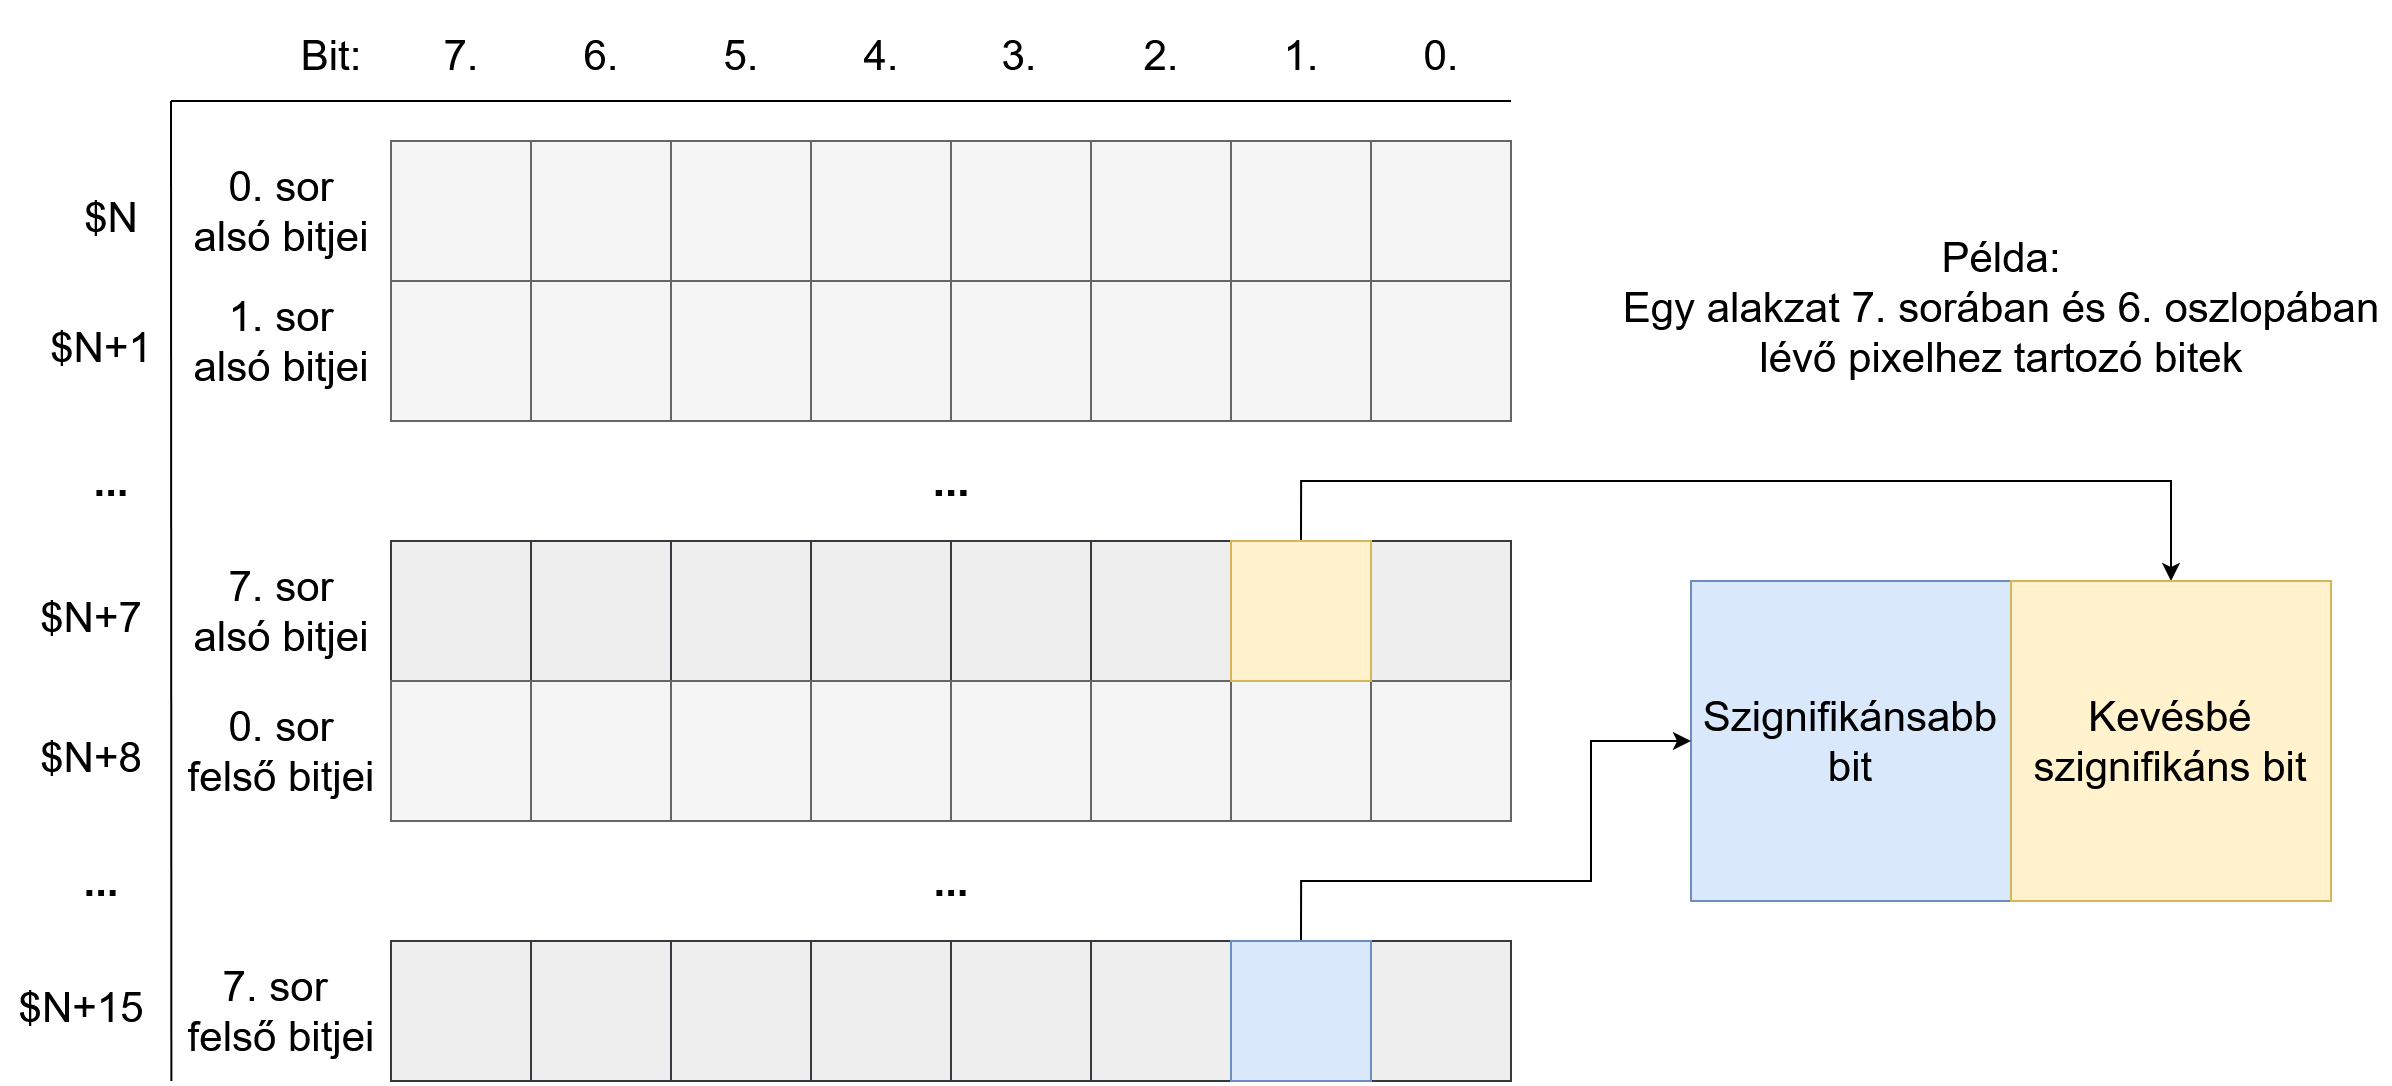
\includegraphics[scale=0.175,frame]{patt.png}
	\caption{Egy alakzat reprezentálása}
	\label{fig:patt}
\end{figure}


\begin{figure}[H]
	\centering
	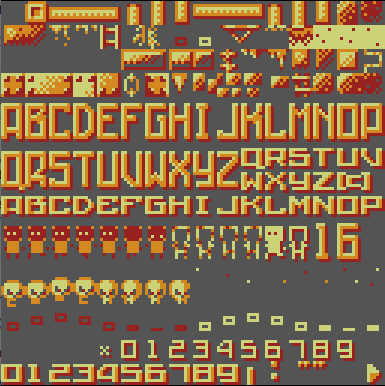
\includegraphics[width=0.45\linewidth,frame]{patt2.png}
	\hspace{5pt}
	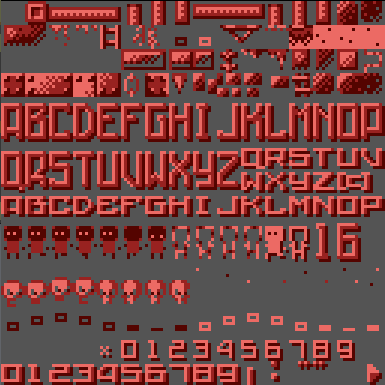
\includegraphics[width=0.45\linewidth,frame]{patt1.png}
	\caption{Az Alter Ego játék 0. alakzattáblázata különböző palettákkal kirajzolva}
\end{figure}

\subsection{Rétegek \cite{ppuref}}
A képfeldolgozó két réteget képes kezelni hardveresen, ezek a háttér és a sprite rétegek.
Általában a képkocka azon részei tartoznak a háttérhez, amik ritkán változnak (például feliratok, számlálók, mozdulatlan képek) és a kirajzolásukhoz nem szükséges további transzformáció (eltolás, tükrözés). A háttérben az alakzatok 30 sorból és 32 oszlopból álló négyzetrácsot alkotnak (ebből és az alakzatok méretéből ered a NES 256*240 pixeles felbontása).
A háttér rétegben egyesével nem lehet alakzatokat eltolni, csak az egész háttér eltolása lehetséges. A sprite rétegben nagyobb flexibilitás áll rendelkezésre, ugyanis itt egyenként, pixel pontosságú eltolással, valamint horizontális és/vagy vertikális tükrözéssel rajzolhatjuk ki az alakzatokat. A sprite rétegnél legfeljebb 64 alakzat szerepelhet egy képkockán (ez a megkötés a később ismertetett OAM méretéből adódik).  

\subsection{Névtáblázatok \cite{ppuref}}

A háttérréteg négyzetrácsának elrendezését a névtáblázatok tárolják. Egy névtáblázat a háttér 960 darab alakzatcellájának mindegyikéhez eltárolja a cellába rajzolandó alakzat sorszámát. Ez a sorszám relatív, ugyanis mindig azon az alakzattáblázaton belül értendő, amit a CONTROLLER regiszterrel a program kiválaszt.

\subsection{Attribútumtáblázatok \cite{ppuref}}

Minden névtáblázathoz tartozik egy 64 bájtos attribútumtáblázat, ami a 960 bájt után következik. Az attribútumtáblázatban minden bájt egy 4*4 alakzatcellából álló terület palettáit határozza meg. A bájtok 4 darab 2 bites részre vannak felosztva, ahol mindegyik rész egy 2*2 cellából álló terület palettájának sorszámát kódolja el (ugyan 8 paletta van, de ebből csak 4 háttérpaletta, így elég 2 bit). Ennek a reprezentációnak a következménye, hogy a háttér 4 cellából álló csoportjai mindig egy palettán osztoznak. A 16 cellát lefedő bájt felosztása a 4 cellás területek között a \ref{fig:attr} ábrán van szemléltetve.

\begin{figure}[H]
	\centering
	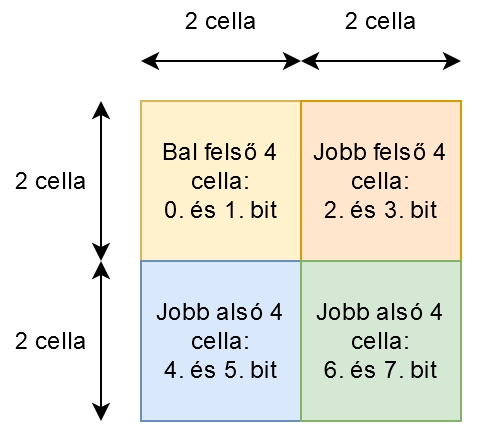
\includegraphics[width=0.45\linewidth]{attrtable.png}
	\caption{Attribútumbájtok felosztása}
	\label{fig:attr}
\end{figure}

\subsection{Háttéreltolás}

A háttéreltolás segítségével pixelpontossággal megszabhatjuk, hogy a háttér mely része legyen látható a játékos számára.
Az eltolás miatt van szükség több névtáblára, ugyanis a lecsúszó háttérrész nem az aktív, hanem háttértükrözéstől függően valamelyik másik névtáblázatból lesz kiolvasva. \cite{memmirror} \cite{scroll}

\subsection{OAM (Object Attribute Memory) \cite{ppuref}}

A sprite réteg elrendezését leíró 256 bájtos memória. 64 darab alakzatról tárol információt, amik a következők:

\begin{compactitem}
	\item X és Y koordináta
	\item A sprite réteg aktív alakzattáblázatán belüli sorszám
	\item Tükrözés
	\item Paletta sorszám
	\item Prioritás a háttérrel szemben
\end{compactitem}

\subsection{Regiszterek \cite{ppuref}}

A CPU és a PPU az alább látható 9 darab egy bájtos regiszter segítségével tud egymással kommunikálni. A regisztereket a CPU a zárójelekben található címeken tudja elérni.
Az olvasató regiszterek \textbf{R}, az írhatók \textbf{W} betűvel vannak megjelölve.

\vspace{0.25cm}

\begin{description}
	\item[CONTROLLER(\$2000, W):] \hfill \\
	A kirajzolás vezérlésére szolgáló regiszter.
	Beállítható vele a következő képkockánál használandó táblázatok indexe.
	\begin{compactdesc}
		\item[0-1. bit:] Aktív névtáblázat indexe
		\item[2. bit:] VRAM cím inkrementálási mód
		\item[3. bit:] Aktív alakzattáblázat indexe a sprite rétegnél
		\item[4. bit:] Aktív alakzattáblázat indexe a háttér rétegnél
		\item[5. bit:] Sprite méret (8x8 vagy 8x16 pixel)
		\item[6. bit:] Az emuláció során nem használt bit
		\item[7. bit:] NMI generálása a PPU tétlen periódusának kezdetén
	\end{compactdesc}
	\item[MASK(\$2001, W):] \hfill \\
	A rétegek egyenkénti ki/bekapcsolása és speciális effektusok 
	(például szürkeárnyalat) vezérelhetők vele.
	\item[STATUS(\$2002, R):] \hfill \\
	A kirajzolás alatt bekövetkező eseményeket jelzi a PPU a CPU-nak ezzel a regiszeterrel.
	Ilyen esemény például a sprite túlcsordulás, ami akkor áll fent, ha több mint a 8 alakzat kerülne egy sorra a sprite rétegben. 
	\item[OAMADDR(\$2003, W) és OAMDATA(\$2004, R/W):] \hfill \\
	A processzor ezen két regiszter segítségével képes új adatokkal feltölteni az OAM memóriát.
	Az alábbi kódrészlet azt szemlélteti, hogy az \emph{adatok} tömb tartalmát hogyan kell a CPU memóriájából
	az OAM-ba átmásolni egy megadott címtől kezdve. Az OAMDATA írása után az OAMADDR automatikusan inkrementálódik a másolás gyorsításának érdekében.
	\begin{lstlisting}
	OAMADDR := 8 bites OAM cim
	for i in 1..adatok.hossz
		OAMDATA := adatok[i]
	\end{lstlisting}
	\item[PPUSCROLL(\$2005, W):] \hfill \\
	Beállíthatjuk vele, hogy a hátteret hány pixellel szeretnénk arrébbcsúsztatni (Horizontális tükrözésnél vízszintesen, vertikális tükrözésnél függőlegesen).
	\item[PPUADDR(\$2006, W) és PPUDATA(\$2007, R/W):] \hfill \\
	A névtáblák frissítésére szolgálnak. Hasonlóan kell őket használni, mint az OAMADDR és OAMDATA regisztereket.
	\item[OAMDMA(\$4014, W):] \hfill \\
	Az OAM memória frissítésének egy alternatív, gyorsabb módja a Direct Memory Access (DMA). Ekkor a processzorban található dedikált hardver másolja át az adatokat egyenesen a CPU RAM-ból az OAM memóriába. A másolás megkezdéséhez annak a memórialapnak a sorszámát kell beírni a regiszterbe, ahol az átmásolandó adatok találhatók.
\end{description}

\subsection{Memóriatérkép \cite{ppuref}}

\begin{table}[H]
	\centering
	\begin{tabular}{ | l | l | }
		\hline
		Tartomány & Paletta \\
		\hline			
		$ \$0000 - \$0FFF $ & 0. Alakzattáblázat \\
		$ \$1000 - \$1FFF $ & 1. Alakzattáblázat \\
		$ \$2000 - \$23FF $ & 0. Névtáblázat \\
		$ \$2400 - \$27FF $ & 1. Névtáblázat \\
		$ \$2800 - \$2BFF $ & 2. Névtáblázat \\
		$ \$2C00 - \$2FFF $ & 3. Névtáblázat \\
		$ \$3000 - \$3EFF $ & A 0-3. névtáblázatok tükrözése \\
		$ \$3F00 - \$3F1F $ & Paletta indexek \\
		$ \$3F20 - \$3FFF $ & Paletta indexek tükrözése \\
		\hline
	\end{tabular}
	\caption{A képfeldolgozó memóriatérképe}
	\label{fig:ppumemmap}
\end{table}

\subsection{A háttér kirajzolásának egyszerű algoritmusa}

Ezen a ponton már minden részletet ismerünk ahhoz, hogy megérthessük a háttérkirajzolás logikáját. A következő pszeudokód azt szemlélteti, hogy a fent említett táblázatokat és a paletta indexet hogyan kell együtt használni a háttér kiszámolásához. Az egyszerűség kedvéért a háttéreltolást itt nem veszem figyelembe. Sajnos ez az algoritmus ebben a formában emulációra nem alkalmas, mert nehézzé teszi a processzor párhuzamos, megfelelő szinkronizációval történő futtatását.
\vspace{0.3cm}

\begin{lstlisting}[backgroundcolor = \color{white}, language=c, basicstyle=\scriptsize]

// Egy bájt indexedik bitjének kiolvasása (0/1)
byte bit(byte bájt, int index)
begin
	return (bájt >> index) & 1
end

// Az alábbi függvénnyel olvassuk a PPU memóriáját (lásd PPU memóriatérkép)
byte olvas(cím)

type RGB_Kód = (byte, byte, byte)

// Palettasorszámból és azonosítósorszámból a szín kikeresése (emlékeztető: $3F00 a paletta index kezdőcíme)
RGB_Kód színKeresés(byte palettaSorszám, byte azonosítóSorszám)
begin
	byte színAzonosító := olvas($3F00 + palettaSorszám*4 + azonosítóSorszám)
	return színPaletta[színAzonosító]
end

// Az eredményül kapott pixeleket tároló kétdimenziós tömb
RGB_Kód pixelek[256][240]

procedure HáttérKirajzol
begin
	// A CONTROLLER regiszterrel a választott névtáblázat
	// és alakzattáblázat kezdőcímének meghatározása
	cím aktívNévtáblazat     := $2000 + (CONTROLLER & 0b11) * $400
	cím aktívAlakzatTáblázat := bit(CONTROLLER, 4) * $1000
	
	// Végigiterálás a háttér celláin
	for cellaSor in 0..29
		for cellaOszlop in 0..31
		begin
		  // A cellához tartozó névtáblabájt indexének kiszámolása
		  byte NTB_Eltolás := cellaSor * 32 + cellaOszlop 
		  
		  // A névtáblabájt kiolvasása
			byte NTB := olvas(aktívNévtáblázat + NTB_Eltolás)
			
			// A cellához tartozó attribútumbájt eltolása a névtábla
			// kezdőcíméhez viszonyítva.
			cím ATB_Eltolás := 
				// Átlépjük a 960 névtáblabájtot 
				$3C0 +		
								
				// Átlépjük az előző cellasorok attribútumbájtjait
				// Emlékeztető: egy sorban 32 alakzat van amik 
				// négyesével osztoznak a bájton
				(cellaSor div 4) * 8 + 	
					
				// Átlépjük a jelenlegi cellasorban az előző attribútumbájtokat
				(cellaOszlop div 4)         
				
			// Az attribútumbájt kiolvasása
			byte ATB := olvas(aktívNévtáblázat + ATB_Eltolás)
			
			// Az attribútumbájtnak a cellához tartozó 2 bites része lesz a palettasorszám.
			// Ki kell számolni, hogy a cella melyik (bal felső, jobb felső, stb.)
			// kvadránsába esik a bájt által lefedett 4*4-es területnek, ugyanis így kapjuk meg,
			// hogy a bájt melyik 2 bitjére van szükségünk
			byte kvadráns := (cellaSor & 0b10)*2 + (cellaOszlop & 0b10) 
			byte palettaSorszám := (ATB >> kvadráns) & 0b11
				
			// Az alakzat kezdőcíme az alakzattáblában
			// Segítség: egy alakzat 16 bájtot foglal
			cim alakzatCím := aktívAlakzatTáblázat + NTB*16
				
			// Végigiterálás a cella 8*8 pixeles területén
			for pixelSor in 0..7
			begin
				cim alakzatSor := alakzatCím + pixelSor
				
				// A sor alsó bitjei
				byte alakzatLSB := olvas(alakzatSor)
				
				// A sor felső bitjei		
				byte alakzatMSB := olvas(alakzatSor + 8)
				
				for pixelOszlop 0..7
				begin
					// A pixelhez tartozó 2 bittel a palettán belüli szín meghatározása
					byte azonosítóSorszám := 
					  (bit(alakzatMSB, 7-pixelOszlop) << 1) | bit(alakzatLSB, 7-pixelOszlop)
					
					// A pixel X koordinátája a képernyőn (0-255)
					byte X := cellaOszlop * 8 + pixelOszlop
					
					// A pixel Y koordinátája a képernyőn (0-239)
					byte Y := cellaSor * 8 + pixelSor
				
					// Az RGB kód kikeresése és beállítása
					pixelek[X][Y] := színKeresés(palettaSorszám, azonosítóSorszám)
				end
			end
		end
end


\end{lstlisting}

\subsection{Sprite réteg kirajzolása}

A kirajzolás algoritmusa annyiban változik, hogy a névtáblázatok és attribútumtáblázatok helyett az OAM memóriát használva határozzuk meg az alakzatsorszámokat és palettasorszámokat.
A 240 sor mindegyikénél a kirajzolás megkezdése előtt ki kell értékelni, hogy melyek azok az alakzatok, amik a következő soron láthatóak. Ezeknek az adatait egy pufferbe, u.n. másodlagos OAM-ba kell helyezni (legfeljebb 8 OAM bejegyzés fér bele). Minden pixelnél megnézzük, hogy van-e olyan alakzat a másodlagos OAM-ban, ami arra a pixelre esik. Ha több is van, akkor a kisebb indexű alakzat élvez nagyobb prioritást. 

\clearpage

\chapter{Fejlesztői dokumentáció II: Megvalósítás} % Developer guide

\section{A feladat specifikációja}

A feladat a NES játékkonzol CPU-ját, PPU-ját és kazettáit valós időben emulálni képes szoftver implementálása, ahol a játékos a játék irányítása mellett képes a virtuális gép állapotának elmentésére és betöltésére, valamint az emuláció vezérlésére. A játékokat billentyűzettel vagy kontrollerrel lehet irányítani. A program felhasználói felülettel is rendelkezik, amivel szintén tudunk mentéseket kezelni és szüneteltethetjük az emulációt.

\section{Fejlesztői környezet}

A programot Haskell nyelven írtam és a GHC 8.10.1-es verziójával fordítottam. Szerkesztőprogramként Visual Studio Code-ot használtam. A Haskell-ben írt függőségi könyvtárak telepítéséhez a Stack\footnote{Haskell Tool Stack: \url{https://docs.haskellstack.org/en/stable/README/}} eszközt használtam.
Az SDL2 és a GTK könyvtárakat Linux-on a disztribúció csomagkezelőjével, Windows-on az MSYS2 konzol csomagkezelőjével telepítettem. 
\clearpage
\subsubsection{Csomagok telepítése}
\begin{itemize}
	\item Windows (MSYS2 konzollal):
	\begin{lstlisting}[language=bash]
	pacman -S mingw-w64-x86_64-SDL2
	pacman -S mingw-w64-x86_64-gtk3
	\end{lstlisting}
	\item Linux:
	\begin{lstlisting}[language=bash]
	$ sudo apt-get install libgirepository1.0-dev
	$ sudo apt-get install libwebkit2gtk-4.0-dev
	$ sudo apt-get install libgtksourceview-3.0-dev
	$ sudo apt-get install libsdl2-dev
	\end{lstlisting}
\end{itemize}

\subsubsection{Fordítás}
\begin{itemize}
	\item Windows: A fordításnál be kell állítani az alábbi környezeti változókat, hogy 
	az MSYS2-vel telepített könyvtárakról tudjon a Stack. A lenti példában az alapértelmezett MSYS2 útvonalakat állítom be.
	\begin{lstlisting}[language=bash]
	SET PATH=C:\msys64\mingw64\bin;C:\msys64\usr\bin;%PATH%
	SET PKG_CONFIG_PATH=C:\msys64\mingw64\lib\pkgconfig
	SET XDG_DATA_DIRS=C:\msys64\mingw64\share
	stack build
	\end{lstlisting}
	Ha az első fordításnál hibát kapunk a \emph{gi-*} függőségek telepítésénél, akkor másoljuk a 
	\emph{C:$\textbackslash$msys64$\textbackslash$mingw64$\textbackslash$bin$\textbackslash$zlib1.dll} fájlt a Stack által telepített GHC \emph{mingw/bin} mappájába. Ha már van ilyen fájl ott, akkor készítsünk róla másolatot, majd cseréljük le.
	\footnote{További információk: \url{https://github.com/haskell-gi/haskell-gi/wiki/Using-haskell-gi-in-Windows}}

	\item Linux:
	\begin{lstlisting}[language=bash]
	$ stack build
	\end{lstlisting}
\end{itemize}

\subsubsection{Futtatás}
A programot a következő paranccsal tudjuk elindítani:
\begin{lstlisting}[language=bash]
stack exec pure-nes
\end{lstlisting}

\section{Az emulációhoz kapcsolódó modulok}

Minden komponenshez (CPU, PPU, kazetták) tartozik egy \emph{Memory} modul, ami definiálja a komponens emulációja során használt rekordokat. A \emph{Serialization} modulok ezen rekordok mentését/betöltését tartalmazzák. A CPU és a PPU \emph{Emulation} moduljai tartalmazzák a hozzájuk tartozó rekordokon végezhető műveleteket.

A \emph{Monad} modul definiálja az emulációs monádot és az abban elérhető primitív műveleteket.
A \emph{MasterClock} modul összefogja a komponenseket és szinkronizálja azok emulációját.
A \emph{Controls} modul a NES sztenderd kontrollerének emulációját tartalmazza.   

A \emph{JoyControls} modul a fizikai kontrollerek kezelését végzi (újonnan csatlakoztatott kontroller és annak rezgőmotorjának inicializálása, gombnyomások megfeleltetése parancsoknak).

Az \emph{AppResources} modulban található rekord az emulátor teljes állapotát tárolja (virtuális gép, shaderek, ablak, stb.).
A \emph{Window} modul az SDL2 multimédia-könyvtárat és az OpenGL-t használva megjeleníti az előállított képkockákat. A \emph{CrtShader} modulban a CRT effektusért felelős OpenGL shaderek találhatók. A \emph{Framerate} modul függvényeivel tudjuk szabályozni a képkockaszámot (fix vagy korlátozatlan számú képkocka/másodperc). A \emph{Logic} modul fogadja az SDL-től érkező gombnyomás-eseményeket, feldolgozza a parancsokat és lépteti az emulációt.

A \emph{Communication} modul definiálja azokat az eseményeket (\emph{Event}), amiket az emulációs ablak a felhasználói felületnek küldhet (mentés/betöltés eredménye, megjelenítendő figyelmeztetés/hibaüzenet), illetve azokat a parancsokat (\emph{Command}), amiket attól fogadhat (szüneteltetés, mentés/betöltés, leállítás, stb.).

\section{A felhasználói felületnél használt technológiák}

A GTK (GIMP Toolkit) egy nyílt forráskódú, kezelőfelületek tervezésére szolgáló szoftvercsomag.
Az API-ja javarészt imperatív stílusú, például a widget-ek létrehozását követően mellékhatásos függvényekkel tudjuk beállítani az attribútumokat és az eseménykezelőket. A Haskellben elérhető \emph{gi-gtk-declarative}\footnote{\url{https://hackage.haskell.org/package/gi-gtk-declarative}} könyvtár ezzel szemben egy deklaratív GTK API-t ad a kezünkbe, aminek segítségével röviden és tömören tudjuk összetett vezérlőelemek megjelenését leírni. 
A \emph{gi-gtk-declarative-app-simple}\footnote{\url{https://hackage.haskell.org/package/gi-gtk-declarative-app-simple}} erre építve definiál felhasználói felületek vezérléséhez egy egyszerű architektúrát, ahol a felületet állapotgépnek tekintjük és az állapotátmeneteket események váltják ki. A felület létrehozásához elég a kezdőállapotot, az állapotmegjelenítő $(state \rightarrow window)$ függvényt és az állapotátmenet-függvényt definiálni.

\section{A felhasználói felülethez kapcsolódó modulok}

\begin{compactdesc}
	\item[A felhasználói felület moduljai]
	\item[State:]
	A felhasználói felület állapotait reprezentáló algebrai adattípus (\emph{State}) definíciója található ebben a modulban. Minden állapothoz tartoznak adatmezők, amik a megjelenítéshez és az állapotátmenetekhez szükséges információkat tárolják (lásd \ref{fig:guistate} ábra).
	\item[InGame:]
	Az emulációs állapot megjelenítéséhez használt segédfüggvényt (\emph{inGame}) tartalmazza, ami az állapot adatmezőiből összeállítja a deklaratív vezérlő-leírást.
	\item[Window:]
	Az \emph{Üzenet}, \emph{Irányítási beállítások} és \emph{Főmenű} állapotok megjelenítéséhez használt segédfüggvényeket (\emph{messageWidget, controlsWidget, startMenu}), valamint a segédfüggvények egyesítésével kapott függvényt (\emph{visualize}) tartalmazza, ami minden állapotot meg tud jeleníteni.
	\item[Logic (Main):]
	Az állapotátmenet-függvényt (\emph{update}) tartalmazza, ami kezeli a felület vezérlőelemeitől vagy az emulációs ablaktól érkező eseményeket, azok hatására frissíti a jelenlegi állapotot, átmegy egy teljesen új állapotba vagy parancsot küld az emulációs ablaknak.
\end{compactdesc}

\begin{figure}[H]
	\centering
	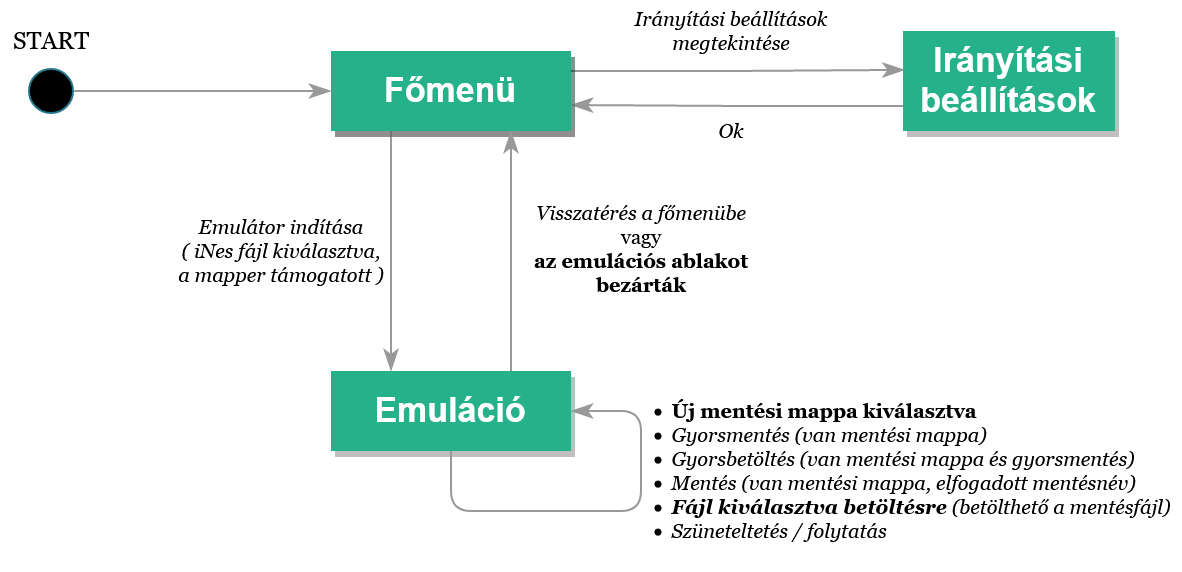
\includegraphics[width=1\linewidth]{statetrans.png}
	\caption{A felület állapotátmenetei}
	\label{fig:states}
\end{figure}

A \ref{fig:states} ábra a felület eseményeit és azoknak állapotváltoztató hatásait hivatott vizualizálni. A dőlt betűs részek gombnyomásokat, a kövér betűs részek eseményeket jelölnek. Ha egy eseménynél a zárójelben lévő feltétel nem teljesül, akkor egy negyedik, \emph{Üzenet} nevű állapotba lépünk, ahol megjelenítjük a hibaüzenetet/figyelmeztetést. Innen az \emph{Ok} gomb lenyomására visszatérünk az előző állapotba. A felület bármelyik állapotban bezárható, ekkor a teljes program terminál (az emulációs ablak is bezárul).

\section{Az emulációt magába záró monád}

A CPU, a PPU, valamint a teljes NES emulációjához érdemes egy monádot bevezetni, hogy ne kelljen mindenhol explicit paraméterként átadni a komponens rekordját. A ReaderT monádtranszformer miatt ez bármely ponton elérhető (olvasható) lesz. A \emph{runEmulator} függvénnyel lefuttathatjuk az emuláció mellékhatásait. Az \emph{emulateSubcomponent} függvény célja, hogy a komponensek emulációját egyesítve lehetséges legyen a teljes rendszer emulációja.
\vspace{0.2cm}
\begin{lstlisting}[language=Haskell, basicstyle=\scriptsize]
import Control.Monad.Reader

newtype Emulator component value 
	= Emulator (ReaderT component IO value) 
	deriving 
	(Functor, Applicative, Monad, MonadIO, MonadReader component)

runEmulator :: c -> Emulator c v -> IO v
runEmulator component (Emulator effect) 
	= runReaderT effect component

emulateSubcomponent :: (c -> s) -> Emulator s v -> Emulator c v
emulateSubcomponent subcomponent (Emulator effect) 
	= Emulator (withReaderT subcomponent effect)
\end{lstlisting}

\section{Adatreprezentáció}

A teljesítmény fontos szempont volt, ezért a regisztereket változtatható és u.n. \emph{unboxed} (közvetlenül az értéket tárolják és nem egy mutatót az értékre) referenciákkal ábrázoltam. Az egyes memóriarészeket (CPU RAM, PRG, CHR, stb...) külön-külön, változtatható és unboxed vektorokkal reprezentálom.

\begin{figure}[H]
	\centering
	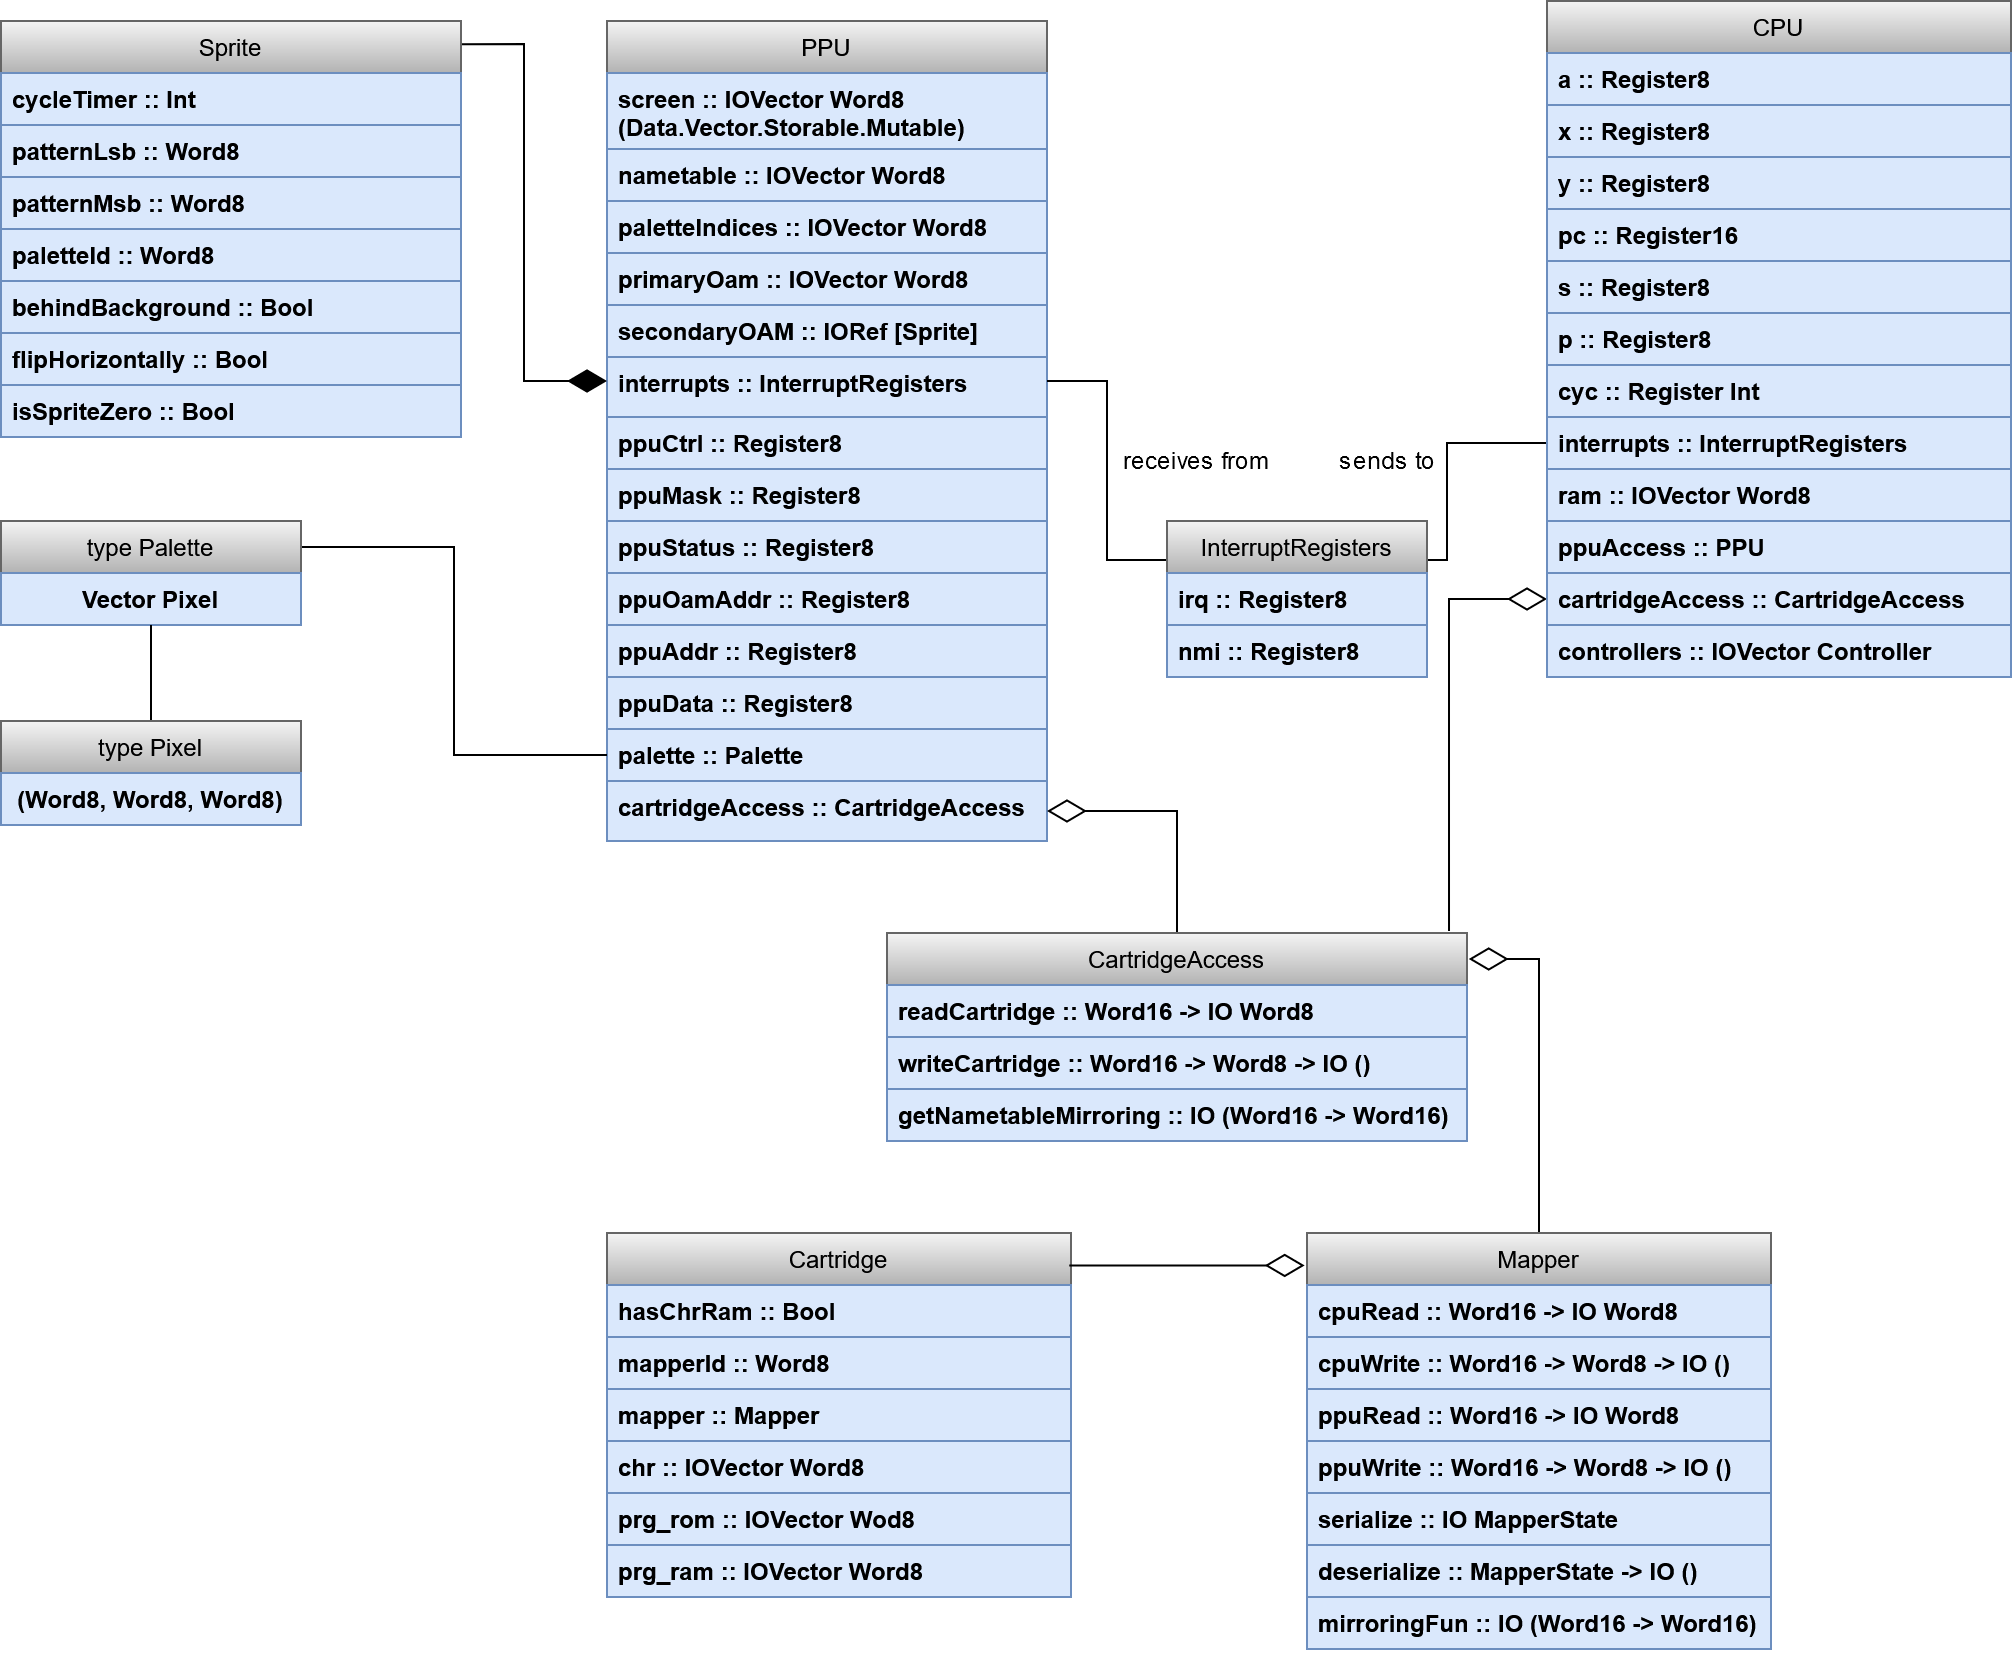
\includegraphics[width=1\linewidth]{data.png}
	\caption{Az emulációnál használt rekordok}
\end{figure}

A CPU és a PPU osztozik a megszakítási "regisztereken", ezért a PPU megszakításokat tud küldeni a CPU-nak.

A kazetta memóriáját a \emph{Cartridge} rekord tárolja. Ehhez közvetlenül nem tudunk hozzáférni, mert a mapper típusa szabja meg, hogy milyen logikájú a címfordítás. A CPU és a PPU a \emph{CartridgeAccess} rekord függvényeit használva tudja olvasni és írni a kazettát, ami a háttérben a megfelelő típusú mapper olvasó és író eljárásait fogja meghívni. A hozzáférést mindkét komponens személyre szabva kapja meg, így tehát a CPU esetében a \emph{readCartridge} függvény a mapper \emph{cpuRead} függvényének felel meg.

\section{Mentés és betöltés}

Ennek a funkciónak a megvalósítása sokféleképp lehetséges. Én egy egyszerű megoldást választottam, ami abból állt, hogy azokhoz a rekordokhoz, amik változtatható referenciákat és vektorokat tartalmaznak, definiáltam egy változtathatatlan (\emph{immutable}) rekordot. A tiszta rekordokhoz automatikusan generálni lehet szerializáló műveleteket (erre a \emph{cereal}\footnote{\url{https://hackage.haskell.org/package/cereal}} könyvtárat használtam), így tehát csak annyi dolgom volt, hogy rekordok közti konverziót implementáljam.
\vspace{0.3cm}
\begin{lstlisting}[language=Haskell]
data SerializedPPU = SerializedPPU {
...
secondaryOam      :: [Sprite],
ppuCtrl           :: Word8,
ppuMask           :: Word8,
...
} deriving (Generic, Serialize)
\end{lstlisting}

\section{Fontos modulok részletes áttekintése}

A program összes modulját és az azok közti függőségeket a \ref{fig:modules} ábrán láthatjuk.

\begin{figure}[H]
	\centering
	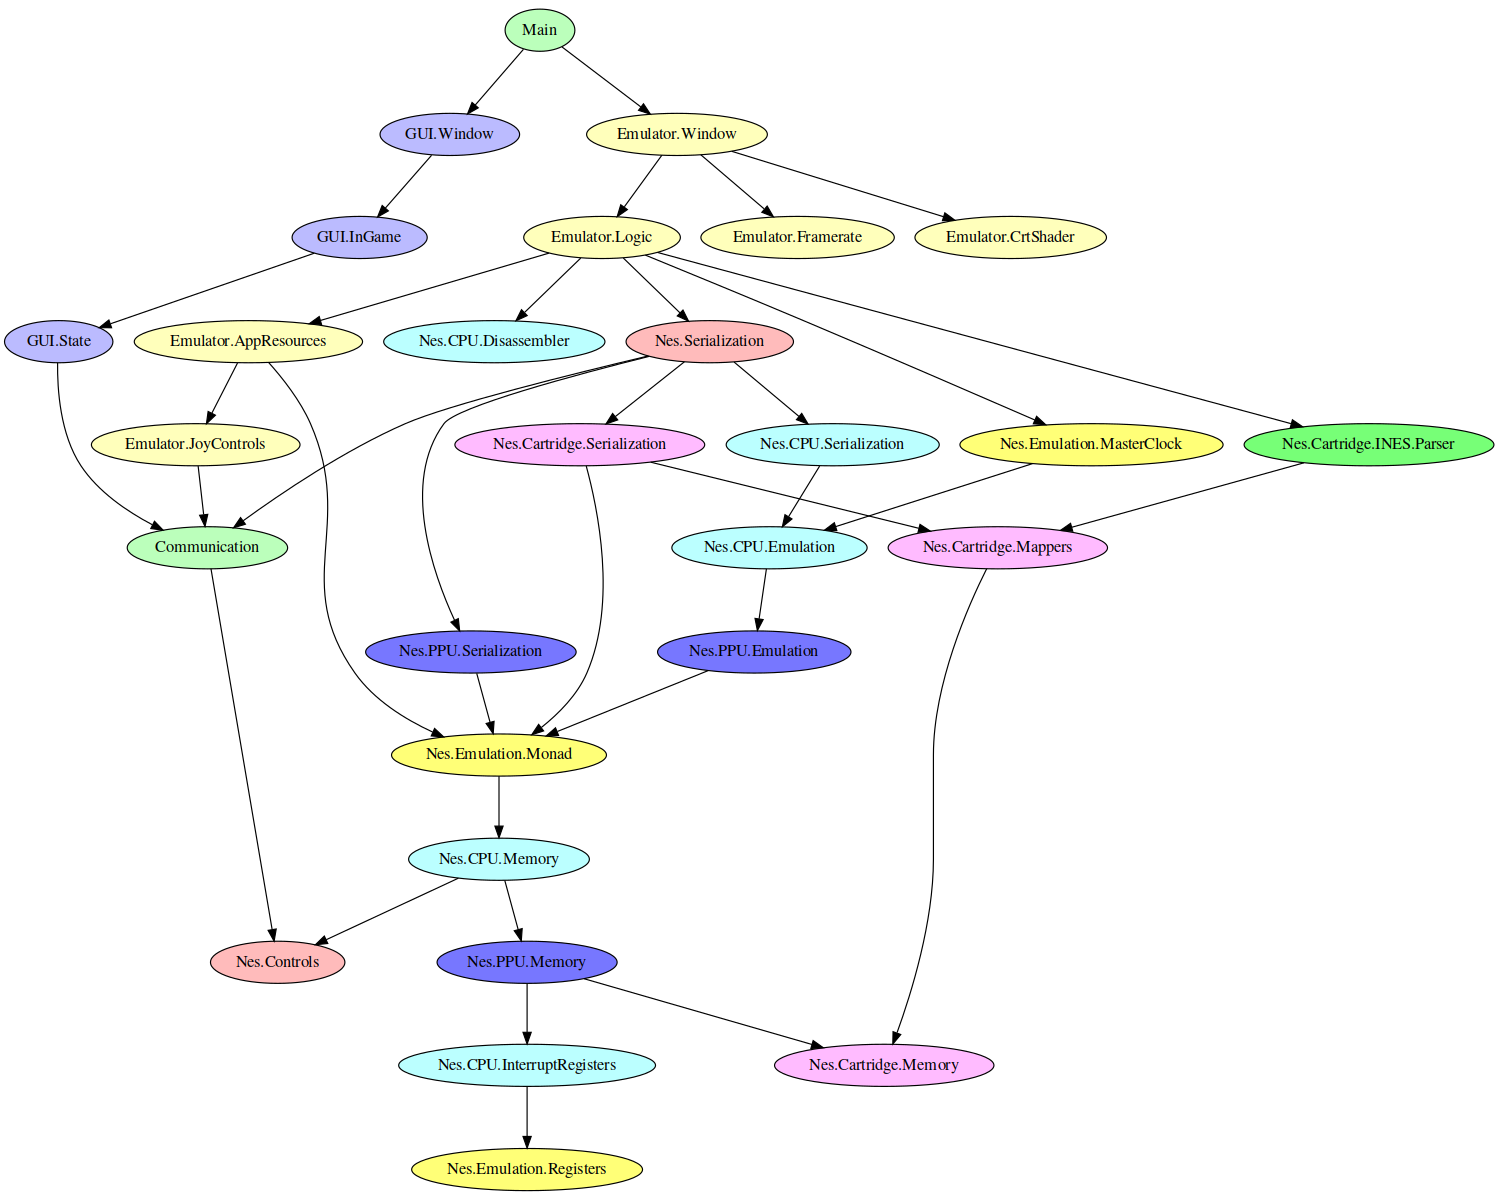
\includegraphics[width=1\linewidth]{modules2.png}
	\caption{A program moduljainak függőségi gráfja}
	\label{fig:modules}
\end{figure}

\subsection{Nes.Cartridge.Memory}
A modul a Cartridge, Mapper és CartridgeAccess rekordok definícióját és a hozzájuk kapcsolódó függvényeket, valamint a névtáblázattükrözési függvényeket tartalmazza.

\begin{description}
	\item[$\bullet\:$ getCPUAccess :: Cartridge $\rightarrow$ CartridgeAccess] \hfill \\
	Hozzáférés kérése a kazettához a CPU számára.
	\item[$\bullet\:$ getPPUAccess :: Cartridge $\rightarrow$ CartridgeAccess] \hfill \\
	Hozzáférés kérése a kazettához a PPU számára.
	\begin{lstlisting}[language=Haskell, basicstyle=\scriptsize]
	getPPUAccess :: Cartridge -> CartridgeAccess
	getPPUAccess Cartridge{mapper=Mapper{ppuRead, ppuWrite, mirroringFunction}} = CartridgeAccess ppuRead ppuWrite mirroringFunction
	\end{lstlisting}
\end{description}

\subsection{Nes.Cartridge.INES.Parser}

Műveletek a kazetta betöltéséhez az iNES fájlból.

\begin{description}
	\item[$\bullet\:$ iNESloader :: Get INES] \hfill \\
	Az iNES fájlokhoz készített parser.
	\item[$\bullet\:$ tryLoadingINES :: FilePath $\rightarrow$ IO INES] \hfill \\
	Az iNES parser futtatása a megadott fájlon, hiba esetén kivétel dobása.
	\item[$\bullet\:$ assembleCartridge :: INES $\rightarrow$ IO Cartridge] \hfill \\
	Az iNES fájl tartalmából az emuláció során használt kazettareprezentáció előállítása.
	\item[$\bullet\:$ loadCartridge :: FilePath $\rightarrow$ IO Cartridge] \hfill \\
	Adott elérési útvonalról egy kazetta betöltése.
	\begin{lstlisting}[language=Haskell]
	import Control.Monad (>=>)
	
	loadCartridge = tryLoadingINES >=> assembleCartridge
	\end{lstlisting}
\end{description}

\subsection{Nes.Cartridge.Mappers}

Ez a modul a mapper-ek implementációit tartalmazza. Ha új mapper-t szeretnénk hozzáadni az emulátorhoz, akkor elég pusztán itt definiálni számára egy konstruktort. A kazetta összeszerelésénél a mapper konstruktora megkapja a félkész kazettát és visszaadja az írásra/olvasásra szolgáló függvényeket tartalmazó rekordot, amik a megfelelő logikával fordítják át a címeket.
A konstruktorok azért nem tiszta függvények, hogy tetszőleges belső állapotot létre lehessen hozni bennük. (a mapper-ek belső regisztereinek száma el szokott térni).

\begin{description}
	\item[$\bullet\:$ mappersById :: Map Word8 (Cartridge $\rightarrow$ IO Mapper)] \hfill \\
	Azonosító $\rightarrow$ konstruktor hozzárendelés. Ha ehhez a Map-hez hozzáadunk egy új mapper konstruktort, akkor azt a mapper-t azonnal támogatottnak érzékeli a betöltő logika.
	\item[$\bullet\:$ nrom  :: Cartridge $\rightarrow$ IO Mapper]
	\item[$\bullet\:$ unrom :: Cartridge $\rightarrow$ IO Mapper]
	\item[$\bullet\:$ cnrom :: Cartridge $\rightarrow$ IO Mapper]
\end{description}

\subsection{Nes.Emulation.Monad}
Az emuláció során használt primitív műveletek.
\begin{description}
	\item[$\bullet\:$ powerUpNes :: Cartridge $\rightarrow$ IO Nes] \hfill \\
	"Behelyezzük" a kazettát és inicializáljuk a komponenseket. 
	\item[$\bullet\:$ useMemory :: (comp $\rightarrow$ ref) $\rightarrow$ (ref $\rightarrow$ IO val) $\rightarrow$ Emulator comp val]
	Kényelmi függvény arra, hogy a komponens rekordjának egy adott mezőjével műveletet végezzünk.
	\begin{lstlisting}[language=Haskell]
	useMemory memory action = asks memory >>= liftIO . action
	\end{lstlisting}
	\item[$\bullet\:$ readMemory és writeMemory]
	Komponens vektorral reprezentált memóriájának közvetlen olvasása és írása (a memóriatérkép nincs figyelembe véve).
	\item[$\bullet\:$ readCartridgeWithAccessor és writeCartridgeWithAccessor]
	A kazettához a CPU-nak és a PPU-nak is saját hozzáférése van, amit ezekkel a függvényekkel tudnak használni.
	\begin{lstlisting}[language=Haskell, basicstyle=\scriptsize]
	readCartridgeWithAccessor :: 
		(component -> CartridgeAccess) -> 
		Word16 -> 
		Emulator component Word8
	writeCartridgeWithAccessor ::
		(component -> CartridgeAccess) -> 
		Word16 ->
		Word8 -> 
		Emulator component ()
	\end{lstlisting}
\end{description}

\subsection{Nes.CPU.Emulation}
A 6502 teljes utasításkészletét tartalmazó modul. Néhány segédfüggvény, eljárás:

\begin{description}
	\item[$\bullet\:$ readReg :: Prim a $\Rightarrow$ (CPU $\rightarrow$ Register a) $\rightarrow$ Emulator CPU a] \hfill \\
	A megadott regiszter olvasása. A regiszterek csak primitív, kicsomagolható típusokat tárolhatnak.
	\item[$\bullet\:$ read :: Word16 $\rightarrow$ Emulator CPU Word8] \hfill \\
	Olvasás a memóriából. A memóriatérkép és a cím alapján dönti el, hogy honnan (RAM, PPU regiszterek, stb...) kell olvasni.
	\item[$\bullet\:$ write :: Word16 $\rightarrow$ Word8 $\rightarrow$ Emulator CPU ()] \hfill \\
	Írás a memóriába. Hasonlóan itt is a memóriatérképet kell figyelembe venni.
	\item[$\bullet\:$ push :: Word8 $\rightarrow$ Emulator CPU ()] \hfill \\
	Bájt felrakása a stack-re.
	\item[$\bullet\:$ pushAddress :: Word16 $\rightarrow$ Emulator CPU ()] \hfill \\
	Cím felrakása a stack-re. Mivel a stack a kisebb címek felé nő, ezért először a szignifikánsabb bájtot kell felrakni, hogy tartsuk a kicsi-az-elején bájtsorrendet.
	\begin{lstlisting}[language=Haskell]
	pushAddress addr = do
		let (high, low) = splitWord16 addr 
		push high
		push low
	\end{lstlisting}
	\item[$\bullet\:$ nmi :: Emulator CPU ()] \hfill \\
	NMI megszakítás érkezésekor meghívott eljárás. Elmenti a programszámlálót és a státusz-regisztert a stack-re és a megszakítási vektor által mutatott címen folytatja a végrehajtást.
	\item[$\bullet\:$ processInterrupts :: Emulator CPU ()] \hfill \\
	Az interrupt-ok nem érkeznek meg azonnal a processzorhoz, hanem időre van szükségük.
	Ennél a virtuális gépnél az interrupt regiszterek tárolják, hogy még hány utasítást kell végrehajtani a megszakításig. A processInterrupts eljárás csökkenti a számlálókat és ha valamelyik számláló eléri a nullát, akkor meghívja a megfelelő megszakítást feldolgozó eljárást. 
	\item[$\bullet\:$ oamDma :: Word8 $\rightarrow$ Emulator CPU ()] \hfill \\
	Adott memórialapról másolás DMA-val a PPU OAM-ba.
\end{description}

\subsection{Nes.PPU.Emulation}

\begin{description}
	\item[$\bullet\:$ cpuReadRegister és cpuWriteRegister] \hfill \\
	A Nes.CPU.Emulation modul számára kiexportált függvények, amivel a CPU kommunikálhat a PPU-val.
	\item[$\bullet\:$ getColor :: Word8 $\rightarrow$ Word8 $\rightarrow$ Emulator PPU Pixel] \hfill \\
	Visszaadja, hogy adott palettán belül adott sorszámú azonosító milyen RGB kódot határoz meg.
	\item[$\bullet\:$ getBackgroundColor :: Emulator PPU (Word8, Word8)] \hfill \\
	Kinyeri a háttér csúsztatóregisztereiből a jelenlegi pixelhez tartozó háttérpaletta sorszámát és az azon belüli indexet.  
	\item[$\bullet\:$ overlaySpriteColor :: (Word8, Word8) $\rightarrow$ Emulator PPU Pixel] \hfill \\
	Kombinálja az háttérszínt a sprite-rétegből származó színnel figyelembe véve a sprite-ok prioritását (háttér előtt/mögött). Az eredmény a pixel végső RGB kódja.
	\item[$\bullet\:$ clock :: Emulator PPU ()] \hfill \\
	A PPU állapotának léptetésére használt függvény. A PPU sorfolytonosan halad végig a képernyőn és állítja elő a pixeleket, amik vagy a háttérrétegből vagy a sprite-rétegből kerülnek ki. Emellett a háttérréteg következő celláinak adatait is előre  betölti.
	A vertikális váltás (a CRT TV elektronágyúja a jobb alsó sarokból visszaáll a bal felső sarokba) ideje alatt tétlen (lásd az időzítési diagramot\cite{frametime}).
\end{description}

\subsection{Nes.Emulation.Controls}

\begin{description}
	\item[$\bullet\:$ press :: Button $\rightarrow$ Controller $\rightarrow$ Controller] \hfill \\
	Ezzel a függvénnyel nyomhatunk le egy gombot a virtuális kontrolleren.
	\item[$\bullet\:$ release :: Button $\rightarrow$ Controller $\rightarrow$ Controller] \hfill \\
	Ezzel a függvénnyel engedhetünk fel egy gombot a virtuális kontrolleren.
	\item[$\bullet\:$ read :: Controller $\rightarrow$ (Word8, Controller)] \hfill \\
		A CPU ezzel a függvénnyel kérdezheti le a kontroller gombjainak állapotát.
		Az $i.$ meghívása a függvénynek visszaadja az $i.$ gomb állapotát. (0 - felengedve, 1 - lenyomva) Az állapotváltoztató hatás a típusból egyértelműen látható.
	\item[$\bullet\:$ write :: Word8 $\rightarrow$ Controller $\rightarrow$ Controller] \hfill \\
		A CPU a kontroller írásával vissza tudja állítani a kontrollert az alaphelyzetbe (a 0. gombot fogja újra a \emph{read} művelet lekérdezni).
	
\end{description}

\subsection{Nes.Emulation.MasterClock}

\begin{description}
	\item[$\bullet\:$ syncCPUwithPPU :: Emulator CPU ()] \hfill \\
	CPU utasítás végrehajtása, majd a megfelelő számú PPU órajel emulálása a szinkronizáció megőrzése érdekében.
	\item[$\bullet\:$ emulateFrame :: Emulator Nes FrameBuffer] \hfill \\
	Addig léptetjük a rendszert az előző függvénnyel, amíg nem végzünk a képkockával.
	\item[$\bullet\:$ resetNes :: Emulator Nes ()] \hfill \\
	Visszaállítja alaphelyzetbe a komponenseket. 
\end{description}

\subsection{Communication}

\subsection{Emulator.JoyControls}

\begin{description}
	\item[$\bullet\:$ init :: ButtonMappings $\rightarrow$ IO JoyControlState] \hfill \\
	Létrehozza azt a rekordot, amiben a gombhozzárendeléseket és csatlakoztatott kontrollereket tartjuk nyilván.
	\item[$\bullet\:$ manageButtonEvent] \hfill \\
	Visszaadja, hogy a gombnyomáshoz milyen parancsok tartoznak (gyorsmentés, gyorsbetöltés vagy játékirányítás). 
	\item[$\bullet\:$ manageHatEvent] \hfill \\
	A DPAD Fel/Le/Balra/Jobbra/Középen eseményeit figyeli és kiadja a megfelelő parancsokat a virtuális kontroller módosítására. Mivel a virtuális kontrollernél nincs Középen állapota a DPAD-nak, ezért arra is figyelni kell, hogy ezt az állapotot \emph{"engedd fel az előző DPAD gombot"} parancsként kell továbbküldeni.
	\item[$\bullet\:$ manageDeviceEvent] \hfill \\
	Figyeli a kontrollercsatlakoztatásokat és az eltávolításokat.
	Az új kontrollereket inicializálja és eltárolja a rekordban, a kihúzottakat eltávolítja.
\end{description}

\subsection{Emulator.Framerate}

\begin{description}
	\item[$\bullet\:$ uncapped :: MonadIO m $\Rightarrow$ m Bool $\rightarrow$ m ()] \hfill \\
	A megadott műveletet futtatja olyan gyorsan, amilyen gyorsan azt lehet addig, amíg a művelet igaz értékkel nem jelzi, hogy terminálni szeretne.
	\item[$\bullet\:$ cappedAt :: MonadIO m $\Rightarrow$ m Bool $\rightarrow$ Word32 $\rightarrow$ m ()] \hfill \\
	A megadott műveletet futtatja a második paraméterben megadott frekvenciával (Hz), amíg a művelet igaz értékkel nem jelzi, hogy terminálni szeretne.
\end{description}

\subsection{Emulator.CrtShader}

\begin{description}
	\item[$\bullet\:$ newShader :: ShaderType $\rightarrow$ ByteString $\rightarrow$ IO Shader] \hfill \\
	Új GLSL shader lefordítása forráskódból. Inkompatibilis OpenGL verziónál előfordulhatnak fordítási hibák, ebben az esetben kivételt dob.
	\item[$\bullet\:$ createProgramFrom :: [Shader] $\rightarrow$ IO Program] \hfill \\
	Linkeli és validálja a shader-ekből készített programot, hiba esetén kivételt dob.
	\item[$\bullet\:$ getCrtShaderProgram :: IO Program] \hfill \\
	A modul exportált eljárása, ami létrehozza a CRT effektust megvalósító shader programot.
	
	\begin{lstlisting}[language=Haskell, basicstyle=\scriptsize]
	import Control.Monad ((=<<), sequence)
	
	getCrtShaderProgram = 
		createProgramFrom =<< sequence 
		[
			newShader VertexShader crtVertexShader, 
			newShader FragmentShader crtFragmentShader
		]
	\end{lstlisting}
\end{description}

\subsection{Emulator.Logic}

\begin{description}
	\item[$\bullet\:$ translateSDLEvent :: SDL.EventPayload $\rightarrow$ Maybe Command] \hfill \\
	Megadja egy beérkező eseményhez a hozzátartozó parancsot.
	\item[$\bullet\:$ pollCommands :: AppResources $\rightarrow$ IO [Command]] \hfill \\
	Lekérdezi az SDL eseményeket és átfordítja őket belső parancsokra. A felhasználói felület által küldött parancsokat kiolvassa az \emph{AppResources}-ban lévő csatornából (\emph{TChan}). A végeredmény a két lista konkatenációja. 
	\item[$\bullet\:$ executeCommand :: AppResources $\rightarrow$ Command $\rightarrow$ Emulator Nes ()] \hfill
	Az eljárás végrehajtja a paraméterül kapott parancsot.
	\item[$\bullet\:$ advanceEmulation :: ViewFunction $\rightarrow$ AppResources $\rightarrow$ Emulator Nes Bool] \hfill
	Végrehajtja az összes parancsot, lépteti az emulációt (ha az nincs szüneteltetve) és a paraméterül kapott megjelenítőfüggvénnyel frissíti a képernyőt.
	\begin{lstlisting}[language=Haskell, basicstyle=\scriptsize]
	type ViewFunction = AppResources -> IOVector Word8 -> Emulator Nes ()
	\end{lstlisting}
\end{description}

\subsection{Emulator.Window}

\begin{description}
	\item[$\bullet\:$ acquireResources :: FilePath $\rightarrow$ CommResources $\rightarrow$ IO AppResources] \hfill Inicializálja az SDL2 és OpenGL könyvtárakat, a létrehozott ablakot, render-ert, kirajzolásnál használt textúrát, stb. visszaadja egy rekordban.
	\item[$\bullet\:$ releaseResources :: AppResources $\rightarrow$ IO ()] \hfill \\
	Felszabadítja a lefoglalt erőforrásokat és leállítja az SDL-t.
	\item[$\bullet\:$ updateScreen :: ViewFunction] \hfill \\
	A paraméterül kapott vektor a megjelenítendő kép nyers pixeladatait tartalmazza RGB24 formátumban. A vektor tartalmát feltölti a videómemóriában tárolt textúrába, majd ezután egy OpenGL (be van kapcsolva a CRT shader és sikerült lefordítani a shader programot) vagy SDL (ki van kapcsolva) hívással kirajzolja a textúrát a képernyőre.
	\item[$\bullet\:$ runEmulatorWindow :: FilePath $\rightarrow$ CommResources $\rightarrow$ IO ()] \hfill \\
	A modul exportált eljárása, amit a grafikus felület indít el egy új szálon. Az emulátor a megadott elérési útvonalról tölti be a kazettát. A második paraméterben kapott csatornákkal tud kommunikálni az felhasználói felülettel.
\end{description}

\section{Egy processzorutasítás végrehajtása}
Ideje, hogy felhasználjuk a Nes.CPU.Emulation modulban implementált tömérdek mennyiségű utasítást. Az első lépés, hogy az utasítás opkódját kiolvassuk.
\vspace{0.3cm}
\begin{lstlisting}[language=Haskell, basicstyle=\scriptsize]
fetch :: Emulator CPU Opcode
fetch = readReg pc >>= read
\end{lstlisting}
\vspace{0.2cm}
Az opkódmátrix segítségével meg kell keresnünk az opkódhoz tartozó utasítást és ciklusszámot. Az opkódmátrix eltárolásának egy egyszerű és meglepően hatékony módja a case elágazás.
\vspace{0.2cm}
\begin{lstlisting}[language=Haskell, basicstyle=\scriptsize]
data DecodedOpcode = DecodedOpcode {
	instruction   :: Emulator CPU (),
	cycles        :: Int
}

decodeOpcode :: Opcode -> DecodedOpcode
decodeOpcode opcode = case opcode of
	0x00 -> DecodedOpcode (implied >> brk) 7;
	...
\end{lstlisting}
\vspace{0.3cm}
Az implementációmnál a dekódolt opkód nem külön, hanem az utasítással "egybeégetve" tartalmazza a címzési módot (így könnyebb volt kezelni azt, hogy nem mindegyik címzési mód ad vissza eredményül címet). A címzési módokat megvalósító függvények arra számítanak, hogy a PC már az opkódot követő bájtra mutat, ezért a végrehajtás előtt meg kell növelni a PC értékét eggyel.
A \emph{cycle} eljárással megnöveljük az eltelt ciklusok számát a statikusan ismert értékkel, az \emph{elapsedCycles} függvénnyel pedig megnézzük, hogy a végrehajtás után ténylegesen hány ciklus telt el.
Így tehát a végső \emph{runNextInstruction} eljárás:
\vspace{0.3cm}
\begin{lstlisting}[language=Haskell, basicstyle=\scriptsize]
import Data.Functor (<&>)

elapsedCycles :: Emulator CPU a -> Emulator CPU Int
elapsedCycles operation = do
	cyclesBefore <- readReg cyc
	operation
	readReg cyc <&> (\cyclesAfter -> cyclesAfter - cyclesBefore)

runInstruction :: DecodedOpcode -> Emulator CPU ()
runInstruction DecodedOpcode{instruction, cycles} = do
	modifyReg pc (+1)
	instruction
	cycle cycles

runNextInstruction :: Emulator CPU Int
runNextInstruction 
 	= elapsedCycles (fetch <&> decodeOpcode >>= runInstruction)
\end{lstlisting}

\section{A CPU és a PPU szinkronizációja}
Az emuláció valójában szekvenciálisan történik, de arra oda kell figyelnünk, hogy egy processzorutasítás végrehajtása után megfelelő számú PPU léptetés történjen meg. Mivel a \emph{runNextInstruction} visszaadja eredményül, hogy hány CPU órajel telt el elméletben az utasítás alatt, így már nem nehéz összehangolni a két komponenst annak tudatában, hogy a PPU órajel-frekvenciája háromszorosa a CPU órajel-frekvenciájának.
A CPU-nak van hozzáférése a PPU-hoz, ezért ezt a CPU szintjén is meg tudjuk tenni.
\begin{lstlisting}[language=Haskell, basicstyle=\scriptsize]
syncCPUwithPPU :: Emulator CPU ()
syncCPUwithPPU = do
	clocks <- CPU.processInterrupts >> CPU.runNextInstruction
	directPPUAccess $ replicateM_ (clocks * 3) PPU.clock
\end{lstlisting}

\section{A grafikus felhasználói felület}
\label{lab:gui}

\subsection{Állapotok}

A felhasználói felület állapotait egy rekurzív algebrai adattípussal modelleztem. A \ref{fig:guistate} ábra mutatja, hogy az adattípusnak milyen konstruktorai vannak és azok milyen mezőkkel rendelkeznek.

\begin{figure}[H]
	\centering
	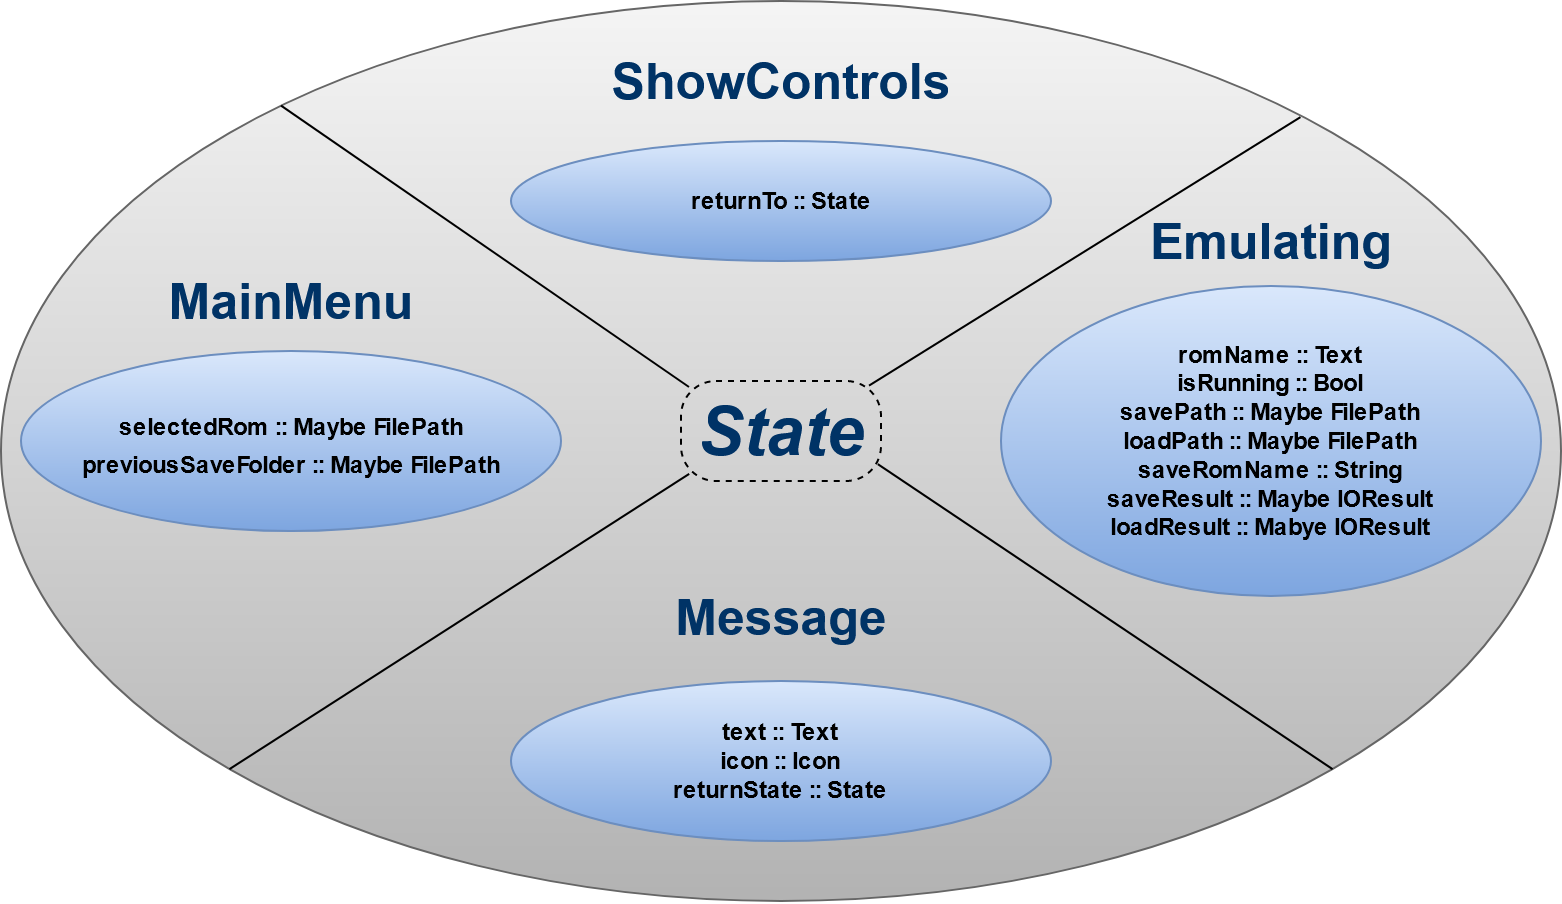
\includegraphics[scale = 0.25]{states.png}
	\caption{A felhasználói felület négy állapota}
	\label{fig:guistate}
\end{figure}

\subsection{Állapotátmenetek}

A mintaillesztési szintaxissal nagyon tömören megfogalmazhatjuk azokat a feltételeket, amiknek teljesülniük kell egy állapotátmenet bekövetkezéséhez.
\vspace{0.2cm}
\begin{lstlisting}[language=Haskell, basicstyle=\scriptsize]
update :: CommResources -> State -> Event -> Transition State Event
update comms Emulating{savePath} ReturnToSelection 
  = Transition (MainMenu Nothing savePath) (sendMsg comms Quit)
\end{lstlisting}
\vspace{0.2cm}
Amikor emuláció közben rányom a felhasználó a főmenübe vezető gombra, akkor a MainMenu állapotba lépünk (és megőrizzük a kiválasztott mentési mappát), mellékhatásként pedig küldünk egy leállási parancsot az emulációs ablaknak a \emph{CommResources} rekordban lévő csatornával. 
\vspace{0.2cm}
\begin{lstlisting}[language=Haskell, basicstyle=\scriptsize]
data MessageIcon = Info | Alert | Cross

saveAsQuick = "You can't name your save as ..."

update _ e@Emulating{saveRomName = "quick"} SaveButtonPressed 
  = Transition (Message saveAsQuick Alert e) noop
\end{lstlisting}

A második példa azt az eshetőséget kezeli, amikor a felhasználó \emph{quick} néven szeretne egyedi mentést létrehozni. Ennek hatására az \emph{Üzenet} állapotba lépünk át ahol megjelenítünk egy figyelmeztető üzenetet (\ref{fig:warning} ábra). Arra is emlékeznünk kell, hogy melyik állapotból jöttünk, hogy később ugyanabba az állapotba térhessünk vissza. 

\begin{figure}[H]
	\centering
	
\includegraphics[scale = 0.9]{alertmsg.png}
	\caption{A kiváltott figyelmeztetés\protect\footnotemark}
	\label{fig:warning}
\end{figure}

\subsection{Állapotmegjelenítés}

\footnotetext{Link az ikonokra: \url{https://www.flaticon.com/packs/ui-interface-23}, \newline \url{https://www.flaticon.com}}
A szemléltetés kedvéért kiragadtam egy részt az \emph{inGame} állapotmegjelenítő-függvényből, ahol azt láthatjuk, hogy a gomb feliratában a játék neve előtt a \emph{Pause} vagy \emph{Resume} szöveg lesz, az állapottól függően.
\vspace{0.2cm}
\begin{lstlisting}[language=Haskell, basicstyle=\scriptsize]
inGame :: State -> Widget Event
inGame Emulating{isRunning, romName} = 
	container Box
	[#orientation := OrientationVertical, #valign := AlignCenter]
	[
		...
	, BoxChild defaultBoxChildProperties $ 
		widget Button
		[ 
			#label :=
			 ((if isRunning then "Pause " else "Resume ") <> romName)
		,	on #clicked TogglePause
		]
		...
	]
	
\end{lstlisting}

A fenti függvény emellett még a következőkről is gondoskodni tud:
\begin{compactitem}
	\item Ha még nincs mentési mappa kiválasztva, akkor ne legyenek kattinthatók az érintett funkciók gombjai
	\item Ha már volt mentési mappa kiválasztva korábbi futtatásnál, akkor a mappaválasztó URI-ját állítsuk be erre
	\item Ha már volt mentési próbálkozás, akkor ikonnal jelezzük a sikerességét, mutassuk az időpontját
	\item Ha már volt betöltési próbálkozás, akkor azt is hasonlóan jelenítsük meg
	\item Szüneteltetésnél és folytatásnál változzon a funkcióhoz tartozó gomb felirata és az ikon
\end{compactitem}

\section{Tesztelés}

A fejlesztés a Test Driven Development (TDD) módszer szerint folyt. Mielőtt belekezdtem volna egy CPU utasítás vagy PPU eljárás implementálásába, a teszteket kibővítettem, hogy az új kódrészeket is lefedjék, ezáltal mindig tudtam, hogy jó irányba haladok-e.

Az emulátorok tesztelésére vannak kifejezetten erre a célre készített NES ROM-ok\footnote{\url{http://wiki.nesdev.com/w/index.php/Emulator_tests}}, amik tökéletes aprólékossággal ellenőrzik, hogy minden utasítás az elvárt módon változtatja-e a hardver belső állapotát. Azért döntöttem ezek használata mellett, mert ilyen pontosságú tesztek írása 6502 Assembly-ben rengeteg időt vett volna el és a saját tesztek lefedettsége meg se közelítette volna a professzionális tesztek által nyújtott lefedettséget.

A tesztek vizuálisan és automatizáltan is futtathatóak. Vizuális futtatásnál a teszt ugyanúgy töltődik be, mint bármilyen más játék és a képernyőre írja ki a teszt eredményét. Automatizáltan futtatni csak előre ismert ROM-okat lehet, mert a tesztek nem egységesek és változó, hogy mivel jelzik az emulátor felé a terminálást, melyik memóriacímen található az eredmény kódja, mit jelentenek a kódok stb.

\subsection{CPU tesztek}

\begin{description}
\item[Nestest] \hfill \\
Részletesen végigteszteli az összes utasítást (beleértve néhány illegálisat is). Az utasítások címzési módját és sorrendjét is variálja. Összesen 8991 utasítást hajt végre. A teszthez tartozó naplóval ellenőrizhetjük, hogy a regiszterek értéke és az eltelt ciklusok száma egyezik-e az elvárttal. 

\item[Instr\_test\_v5] \hfill \\
16 tesztet tartalmaz, amik a címzési módokat, veremműveleteket, elágazásokat és megszakításokat tesztelik. Remek hibaüzeneteket ír a \$6004 címtől kezdve egy nullával terminált sztring segítségével.

\item[Instr\_Misc] \hfill \\
Az abszolút indexelt címzés és az elágazások szélsőséges eseteinek ellenőrzése.

\end{description}

\subsection{PPU tesztek}

\begin{description}
\item[PPU\_vbl\_nmi] \hfill \\
Ez a tesztcsomag a vertical blanking period státusz-flaget (be/kikapcsolása megfelelő időben történik), az NMI megszakítást (bekövetkezik-e, a PPU regiszterek befolyásolják-e) és a páros-páratlan képkockák 1 PPU órajelciklusnyi hosszkülönbségét ellenőrzi.

\item[PPU\_sprite\_hit és PPU\_sprite\_overflow] \hfill \\
12 tesztcsomag, amik a sprite réteggel kapcsolatos státusz flag-eket ellenőrzik (Sprite 0 Hit, Sprite Overflow).

\end{description}

\subsection{Eredmények}

Emulátoroknál a 100\%-os pontosság elérése nehéz feladat, mert az áramkörök felépítéséből természetes következményként adódó speciális viselkedéseket mesterségesen, összetett feltételek ellenőrzésével kell implementálni (például memóriabusz-konfliktus, NMI elnyomás, stb.).  Az emulátorom időzítésekben és az előbb említett két esetben tér el minimálisan az eredeti hardvertől. Összességében a pontosság kielégítő, és a legtöbb játéknál nem okoz gondot az eltérés.

\vspace{0.2cm}
\begin{figure}[H]
	\centering
	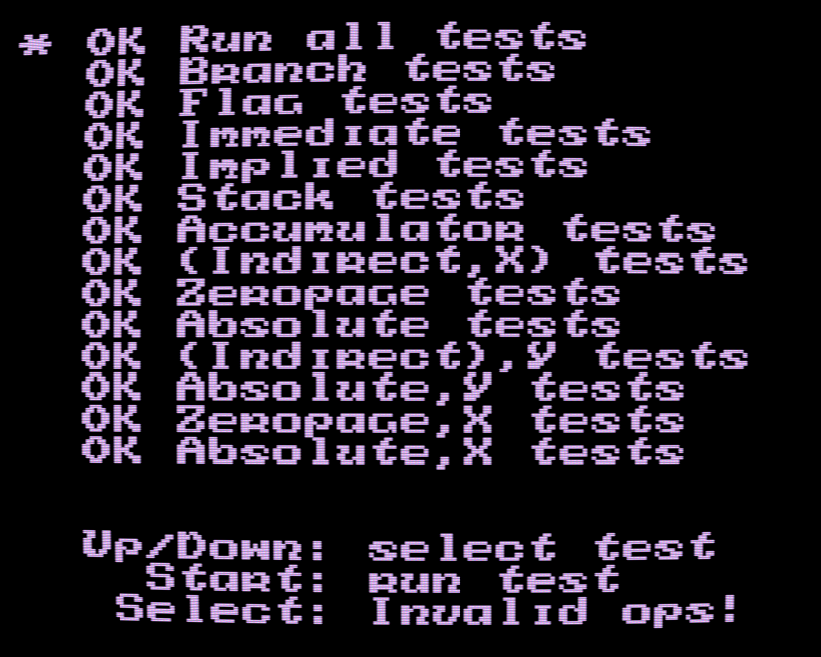
\includegraphics[scale=0.5]{nestest.png}
	\caption{CPU ellenőrzése a Nestest ROM-mal}
\end{figure}


\begin{figure}[H]
	\centering
	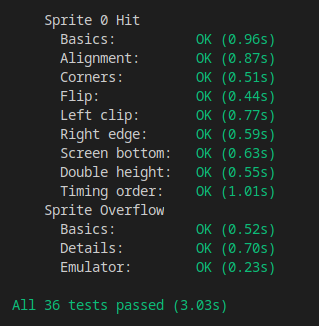
\includegraphics[scale=0.6]{tests.png}
	\caption{Automatizáltan végrehajtott sprite-réteg tesztek}
\end{figure}

\subsection{Tesztelt, megbízhatóan működő programok}

\subsubsection{Játékok}
\begin{compactitem}
	\item Game of Life: \url{https://www.romhacking.net/homebrew/48/}
	\item 2048: \url{https://www.romhacking.net/homebrew/65/}
	\item Alter Ego: \url{https://www.romhacking.net/homebrew/1/} \label{alter}
	\item Lawn Mover: \url{http://www.romhacking.net/homebrew/42/} \label{lawn}
	\item Lan Master: \url{https://www.romhacking.net/homebrew/2/}
	\item Sudoku: \url{https://www.romhacking.net/homebrew/17/}
	\item Chase: \url{https://www.romhacking.net/homebrew/73/}
	\item Chicken Of The Farm: \url{https://www.romhacking.net/homebrew/109/}
	\item Falldown: \url{https://www.romhacking.net/homebrew/57/}
	\item Fighter F8000: \url{http://nesdev.com/fighter\_f8000.zip}
	\item Magic Floor: \url{https://www.romhacking.net/homebrew/40/}
	\item Pegs: \url{https://www.romhacking.net/homebrew/22/}
	\item Pong 198x: \url{https://www.romhacking.net/homebrew/26/}
	\item NeSnake: \url{https://www.romhacking.net/homebrew/31/}
	\item NeSnake 2: \url{https://www.romhacking.net/homebrew/30/}
	\item MilionNESy: \url{https://www.romhacking.net/homebrew/36/}
	\item Sokoban: \url{http://nesdev.com/sokoban.zip}
	\item Concentration Room: \newline \url{http://wiki.nesdev.com/w/index.php/Concentration_Room}
	\item Eskimo Bob Demo: \newline \url{https://spoony-bard-productions.itch.io/eskimo-bob}
\end{compactitem}

\subsubsection{Techdemók}
\begin{compactitem}
	\item Raster Demo: \url{http://nesdev.com/rstrdemo.zip}
	\item Motion \url{http://nesdev.com/anims.zip}
	\item Fullscreen Demo \url{http://nesdev.com/FullScreen.zip}
	\item Interlacing Demo \url{http://nesdev.com/interlac.zip}
\end{compactitem}



